\documentclass[myclassdoc,debug]{rjparticle}
%use the following command when typesetting your paper:
%\documentclass{rjparticle}
\usepackage{graphicx}

\title{Extensive Study of the Positive and Negative Parity Wobbling States for an Odd-Mass Triaxial Nucleus Ii: Geometrical Interpretation} 

\author[1,2,$a$]{R. Poenaru}
\author[2,3,$b$]{A. A. Raduta}

\affil[1]{Doctoral School of Physics, University of Bucharest, Bucharest, Romania\\
\email[a]{robert.poenaru@drd.unibuc.ro} }
\affil[2]{Department of Theoretical Physics - \textit{Horia Hulubei} National Institute for Physics and Nuclear Engineering, M\u{a}gurele-Bucharest, Romania\\
\email[b]{raduta@nipne.ro} (corresponding author)}
\affil[3]{Academy of Romanian Scientists, Bucharest, Romania}

\keywords{Nuclear Structure, Triaxial Nuclei, Wobbling Motion, Parity Symmetry, Signature Partners, Strong Deformation}

\pacs{01.30.-y, 01.30.Ww, 01.30.Xx, 99.00.Bogus}

\hyphenation{rjp-ar-ti-cle}

%%%%%%%%%%%%%%%%%%%%%%%%%%%%%%%%%%%%%%%%%%%%%%%%%%%%%%%%%%%%%%%%%%%%%%%%%%%%%%%
%Please, do not remove the following lines!
%%%%%%%%%%%%%%%%%%%%%%%%%%%%%%%%%%%%%%%%%%%%%%%%%%%%%%%%%%%%%%%%%%%%%%%%%%%%%%%
%\RJPVolume{63}{2018}
%\RJPNumber{1-2}
%\RJPPages{}{}
%\columntitle{Wobbling Nucleus II}
%\date{}
%\dedication{}
%\domaintitle{}
%\keywords{}
%\pacs{01.30.-y, 01.30.Ww, 01.30.Xx, 99.00.Bogus}
%%%%%%%%%%%%%%%%%%%%%%%%%%%%%%%%%%%%%%%%%%%%%%%%%%%%%%%%%%%%%%%%%%%%%%%%%%%%%%%

\begin{document}
%%%%%%%%%%%%%%%%%%%%%%%%%%%%%%%%%%%%%%%%%%%%%%%%%%%%%%%%%%%%%%%%%%%%%%%%%%%%%%%
%Please, remove these lines when typesetting your document!
%%%%%%%%%%%%%%%%%%%%%%%%%%%%%%%%%%%%%%%%%%%%%%%%%%%%%%%%%%%%%%%%%%%%%%%%%%%%%%%
\lstset{%
basicstyle=\small,
language=[AlLaTeX]TeX,
columns=fullflexible,
%keepspaces=true,
showspaces=true,
showstringspaces=false,
keywordstyle=[2]\ttfamily,
identifierstyle=,
texcsstyle=*\ttfamily,
commentstyle=\color{gray},
string=[s]<>,
morestring=[b]',
stringstyle=\emph,
breaklines=true,
deletekeywords={list},
moretexcs={authnote,keywords,pacs},
}
%%%%%%%%%%%%%%%%%%%%%%%%%%%%%%%%%%%%%%%%%%%%%%%%%%%%%%%%%%%%%%%%%%%%%%%%%%%%%%%

\maketitle

\begin{abstract}
A new interpretation of the wobbling structure in $^{163}$Lu is developed. Four wobbling bands are experimentally known in this isotope, where three are wobbling phonon excitations $TSD_{2,3,4}$, and the ground state band, which is $TSD_1$. In this work, a particle-triaxial rotor coupling is considered in a product space of single-particle and collective core states. The single-particle states describe a $j=i_{13/2}$ proton, while the core states characterize the triaxial rotor and are either of positive parity, when the bands $TSD_{1,2,3}$ are concerned or of negative parity for the $TSD_4$ band. There are five free parameters, three moments of inertia, the strength of the particle-core interaction, and the $\gamma$ deformation. A very good description of all 62 experimental states is obtained, with a mean square error of about $80\ \text{keV}$. The newly obtained features evidenced in the present work enrich the knowledge about the wobbling properties of $^{163}$Lu.
\end{abstract}

\section{Introduction compatibility}
\textbf{To be implemented...}
\section{Wobbling motion in nuclei - experimental \& theoretical overview}
\label{section2-wm}

W.M. can be viewed as the quantum analogue for the motion of the asymmetric top, whose rotation around the axis with the largest MOI is energetically the most favored. A uniform rotation about this axis will have the lowest energy for a given angular momentum (spin). As the energy increases, this axis will start to precess with a harmonic type of oscillation about the space-fixed angular momentum vector, giving rise to a family of wobbling bands, each characterized by a wobbling phonon number $n_w$. The resulting quantal spectrum will be a sequence of rotational $\Delta I=2$ bands, with an alternating signature number for each wobbling excitation. According to \cite{bohr1998nuclear}, it is possible to obtain the wobbling spectrum of any triaxial rigid rotor, by using the information related to its angular momentum $I$, moments of inertia $\mathcal{I}_{1,2,3}$, rotational frequency $\omega_\text{rot}$, wobbling frequency $\omega_\text{wob}$ as follows:
\begin{align}
    E_\text{rot}=\sum_i\left(\frac{\hbar^2}{2\mathcal{I}_k}\right)I^2_k\approx\frac{\hbar^2}{2\mathcal{I}_1}I(I+1)+\hbar\omega_\text{wob}\left(n_w+\frac{1}{2}\right)\ , \label{wobbling_eq}
\end{align}
with $\omega_\text{wob}$ given by the following expression:
\begin{align}
    \hbar\omega_\text{wob}=\hbar\omega_\text{rot}\sqrt{\frac{(\mathcal{I}_1-\mathcal{I}_2)(\mathcal{I}_1-\mathcal{I}_3)}{\mathcal{I}_2\mathcal{I}_3}}\ ,
\end{align}
where the rotational frequency of the rigid rotor is given by $\hbar\omega_\text{rot}=\frac{\hbar I^2}{\mathcal{I}_1}$. In Eq. \ref{wobbling_eq}, the approximation of very large MOI along 1-axis is considered (i.e., $\mathcal{I}_1>>\mathcal{I}_2,\mathcal{I}_3$), and $I(I+1)=I_1^2+I_2^2+I_3^2$. One can see that the wobbling motion is expressed as a 1-dimensional vibration with only one variable, since the energy of the zero-point fluctuation is $\frac{\hbar\omega_\text{wob}}{2}$ \cite{hagemann2003quantized}.

\begin{figure}
\centering
\begin{minipage}{.6\textwidth}
  \centering
  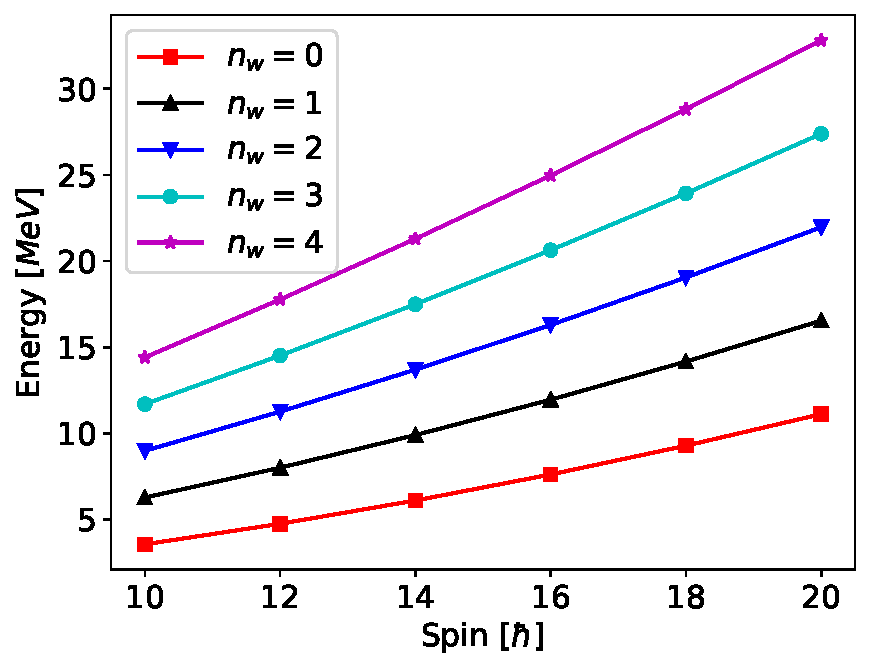
\includegraphics[width=1\linewidth]{figs/simple_wobbling_spectrum.pdf}
  %  \caption{A family of wobbling bands for a triaxial rigid rotor (schematic representation). The calculations were done for $\mathcal{I}_1:\mathcal{I}_2:\mathcal{I}_3=25:5:2$.}
    % \label{simple-wobbling-family}
\end{minipage}%
\begin{minipage}{.4\textwidth}
  \centering
 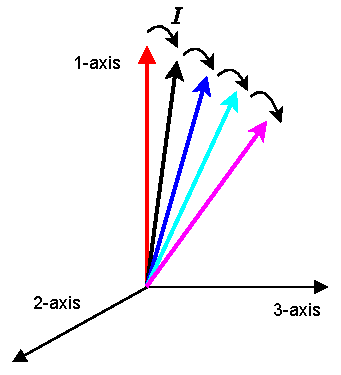
\includegraphics[width=0.85\linewidth]{figs/wobbling_tilting_axis.pdf}
   % \caption{Tilting of the angular momentum away from the rotational axis, with increase in the wobbling phonon excitation.}
    % \label{wobbling-tilt}
\end{minipage}
\caption{Family of wobbling bands for a simple triaxial rotor (left-side). Tilting of the angular momentum vector away from the rotational axis with an increase in spin (right-side). This schematic representation was done for an arbitrary set of MOIs $\mathcal{I}_1:\mathcal{I}_2:\mathcal{I}_3=25:5:2$.}
\label{simple-wobbling-family}
\end{figure}

Just for an illustrative purpose, Figure \ref{simple-wobbling-family} shows a theoretical spectrum for the wobbling bands within a triaxial rigid rotor. The family of wobbling bands is obtained from a set of three moments of inertia (along the three principal axes), a given angular momentum, and increasing wobbling phonon numbers ($n_w=0,1,\dots$). Moreover, in Figure \ref{simple-wobbling-family}, the tilting of the angular momentum away from the rotational axis is sketched, where the tilt increases with the increase in the wobbling excitation. In a given sequence of wobbling bands, both the intra-band $\Delta I=2$ as well as inter-band $\Delta I=1$ transitions have a strong $E2$ collective character.

It is important to mention that the wobbling spectrum described by Eq. \ref{wobbling_eq} and graphically represented in Figure \ref{simple-wobbling-family} was firstly predicted for an even-even triaxial nucleus \cite{bohr1998nuclear}. This predicted wobbling mode has not been experimentally confirmed yet. However, the first experimental evidence for wobbling excitations in nuclei was for an even-odd nucleus, namely $^{163}$Lu, where a single one-phonon wobbling band was measured initially \cite{odegaard2001evidence}, followed by two additional wobbling bands discovered one year later \cite{jensen2002evidence,jensen2002wobbling}.

\subsection{Experimental findings} \label{section2:expdata}

After the first discovery of wobbling bands in $^{163}$Lu ($Z=71$), an entire series of even-odd isotopes with $A\approx160$ were experimentally confirmed as \emph{wobblers}: $^{161}$Lu, $^{165}$Lu, $^{167}$Lu, and $^{167}$Ta. In these nuclei, the wobbling mode appears due to the coupling of a valence nucleon (the so-called $\pi(i_{13/2})$ intruder) to a triaxial core, driving the entire nuclear system up to large deformation ($\epsilon\approx0.4$) \cite{schnack1995superdeformed}.

With time, several nuclei in which WM occurs were also found in regions of smaller $A$. Indeed, two isotopes with $A\approx130$: $^{133}$La \cite{biswas2019longitudinal} and $^{135}$Pr \cite{matta2017transverse,sensharma2019two} were identified as having wobbling bands which emerge from the coupling of a triaxial even-even core with the $\pi(h_{11/2})$ nucleon for $^{135}$Pr, and an additional pair of positive parity quasi-protons for $^{133}$La. In the case of $^{133}$La, the system is characterized as a longitudinal wobbler (it is in fact the first nucleus in which the longitudinal wobbling regime has been experimentally identified), while $^{135}$Pr has a transverse wobbling regime. In both cases, the resulting coupling has a deformation $\epsilon=0.16$ \cite{matta2017transverse,biswas2019longitudinal}, which is smaller than the deformation in the heavier nuclei from the $A\approx160$ region. A third nucleus that also lies in this mass region was confirmed very recently by Chakraborty et. al. in \cite{chakraborty2020multiphonon}, namely the odd-$A$ $^{127}$Xe, where a total of four wobbling bands have been reported by the team (two yrast bands, and two excited phonon bands with $n_w=1$ and $n_w=2$). It is also suggested that $^{131}$Ba could exhibit transverse wobbling \cite{petrache_2018} due to the alignment of a quasiparticle with hole-like character (the $h_{11/2}$ neutron), but in order to support this interpretation, the connecting transitions must show predominant $E2$ character.

Some additional progress was made in the $A\approx100$ mass region, with experimental evidence for $^{105}$Pd with two such bands that are built on a $\nu(h_{11/2})$ configuration, the first one so far in which a valence neutron couples to the triaxial core \cite{timar2019experimental}. The resulting configuration drives the nuclear system up to deformation $\epsilon\approx0.26$ and a transverse wobbling behavior.

The heaviest nuclei known so far in which WM has been experimentally observed are the isotopes $Z=79$ with $A=183$ \cite{nandi2020first} and $A=187$ \cite{sensharma2020longitudinal}, respectively. However, for the case of $^{187}$Au, there is an ongoing investigation \cite{guo2020risk} whether the two wobbling bands ($n_w=0$ and $n_w=1$) are bands with wobbling character, or if they are of magnetic nature (which would exclude the wobbling phonon interpretation). The nucleus $^{183}$Au has probably the most interesting wobbling behavior, due to the appearance of both increasing and decreasing parts of the wobbling energy as a function of angular momentum, for states belonging to the same band (see Figure 5 from \cite{nandi2020first}). The experimental evidence for this nucleus shows that the positive parity band behave as a TW (despite the increasing behavior) due to the geometry of the coupling of the odd quasiparticle. This has important implications which will be discussed later on. For now, it is important to remember that there are cases where some transverse wobblers could be increasing functions of angular momentum, in the low-spin regions.

Regarding the wobbling motion for the even-even nuclei (behavior that was described in Figure \ref{simple-wobbling-family}), the experimental results are fragmentary, with scarce or unclear evidence on this collective behavior. However, some embryos of even-even wobblers have been reported in the recent years. For example, the $^{112}$Ru ($Z=44$) nucleus has three wobbling bands \cite{hamilton2010super}, two of them being the excited one- and two-wobbling phonon bands. Another nucleus is $^{114}$Pd \cite{luo2013triaxial}, with two excited bands of wobbling character, similar to $^{112}$Ru. Indeed, for $^{112}$Ru and $^{114}$Pd the ground band together with the odd and even spin members of the $\gamma$-bands were interpreted as zero-(yrast), one-, and two-phonon wobbling bands. Unfortunately, since there are no data concerning the electromagnetic transitions, its wobbling character is still unclear. The even-even nucleus $^{130}$Ba ($Z=56$) \cite{petrache2019diversity,wang2020two,chen2019transverse} was confirmed very recently to exhibit wobbling behavior based on a two quasiparticle configuration with pair of bands with even and odd spins as zero- and one-phonon wobbling bands, respectively. What is worth noting for this case is the fact that these two bands are built on a configuration in which two aligned protons that emerge from the bottom of $h_{11/2}$ shell couple with the triaxial core. One remarks the change in nature of the wobbling motion from a purely collective form, but in the presence of two aligned quasiparticles \cite{wang2020two}, with a transverse wobbling character. 

Concerning the interpretation of the energy spectrum for the wobbling motion which occurs in the nuclei that were mentioned above, it is mandatory to discuss some aspects related to its behavior with the increase in total angular momentum (nuclear spin). Thus, the concepts of \emph{longitudinal wobblers} (LW) and \emph{transverse wobblers} (TW) emerged from an extensive study done by Frauendorf et. al. \cite{frauendorf2014transverse} in which the team studied the possible coupling schemes that a valence nucleon can create with the triaxial core, giving rise to two possible scenarios. Based on microscopic calculations using the Quasi-Particle Triaxial Rotor (QTR) model, they showed that if the odd valence nucleon aligns its angular momentum vector $\vec{j}$ with the axis of largest MOI, the nuclear system is of longitudinal wobbling character. On the other hand, if the odd nucleon aligns its a.m. vector $\vec{j}$ with an axis perpendicular to the one with the largest MOI, then the nuclear system has a transverse wobbling character. Consequently, for LW the wobbling energy $E_\text{wob}$ (see Eq. \ref{wobbling-energy-relative}) has an \emph{increasing} behavior with an increase in the angular momentum, while for TW the energy $E_\text{wob}$ \emph{decreases} with increasing angular momentum.

From the nuclei that were mentioned above, most of them are of TW type, with only $^{127}$Xe \cite{chakraborty2020multiphonon}, $^{133}$La \cite{biswas2019longitudinal}, and $^{187}$Au \cite{sensharma2020longitudinal} having an LW character. The energy that characterizes the type of wobbling in a nuclear system is the energy of the first excited band (the one-phonon $n_w=1$ wobbling band) relative to the yrast ground band (zero-phonon $n_w=0$ wobbling band):
\begin{align}
    E_\text{wob}(I)=E_{1}(I)-\left(\frac{E_0(I+1)+E_0(I-1)}{2}\right)\ ,
    \label{wobbling-energy-relative}
\end{align}
with 0 and 1 representing the wobbling phonon number $n_w$.

The odd nucleons that couple with the rigid triaxial core will influence the appearance of a particular wobbling regime (LW or TW). In all the wobblers, there is a proton from a certain orbital that is coupling with the core, except for the case of $^{105}$Pd, where the valence nucleon is a neutron. The nature of the odd quasiparticle (i.e., particle or hole) and its "position" in the deformed $j$-shell (i.e., bottom or top) will determine whether its angular momentum $\vec{j}$ will align with the \emph{short} ($s$) or \emph{long} ($l$) axes of the triaxial rotor, respectively (with the notations short $s$, long $l$, and medium $m$ for the axes of a triaxial ellipsoid). The reasoning behind this has to do with the minimization of the overall energy of the system: in the first case, a maximal overlap of its density distribution with the triaxial core will determine a minimal energy, while in the second case, a minimal overlap of the density distribution of the particle with the core will result in a minimal energy. Moreover, if the quasiparticle emerges from the middle of the $j$-shell, then it tends to align its angular momentum vector $\vec{j}$ with the \emph{medium} ($m$) axis of the triaxial core. Figure \ref{quasiparticle-alignment} aims at depicting the type of alignment of a quasiparticle with the triaxial core.

\begin{figure}
    \centering
    % 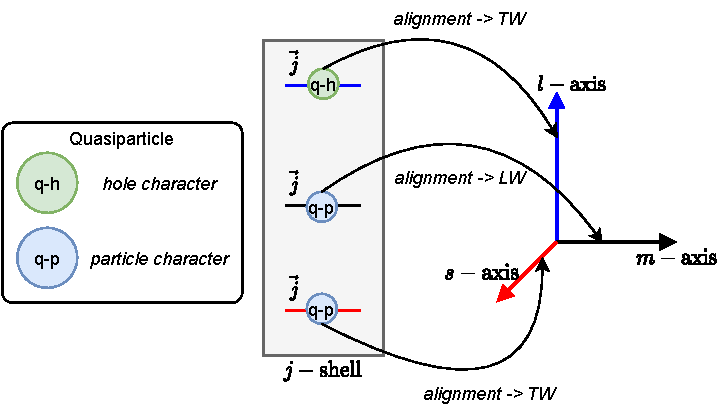
\includegraphics[width=0.85\textwidth]{figs/wobbling_Regimes.pdf}
    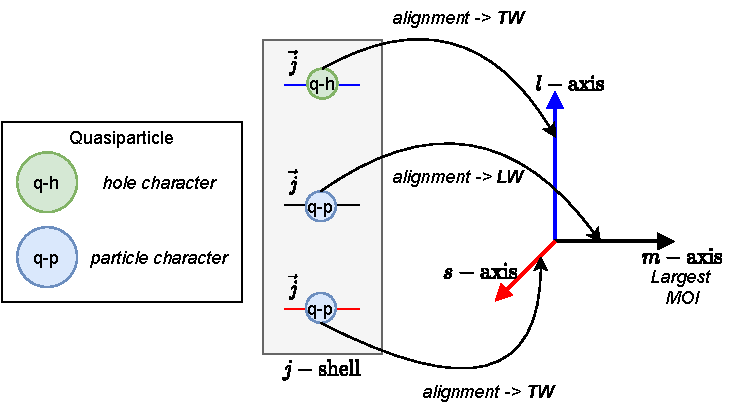
\includegraphics[scale=0.95]{figs/wobbling_Regimes_updated.pdf}
    \caption{The wobbling regimes, Longitudinal Wobbling (LW) or Transverse Wobbling (TW), based on the type of alignment that an odd quasiparticle makes with the principal axes of a triaxial core. Each case depicts a coupling with an odd quasiparticle which emerges from the bottom/middle/top of a $j$-shell \cite{frauendorf2014transverse}.}
    \label{quasiparticle-alignment}
\end{figure}

As previously mentioned, for a given angular momentum, uniform rotation around the axis with the largest MOI corresponds to minimum energy. For a triaxial rotor emerging from a Liquid Drop, this is equivalent to rotation around the $m$ axis. Therefore, Frauendorf \cite{frauendorf2014transverse} classified the LW as the situation when the odd nucleon will align its angular momentum along the $m$-axis, while TW being the situation where $j$ is aligned perpendicular to the $m$-axis (with $s$- or $l$-axis alignment depending on the $j$-shell orbital from which the odd nucleon arises). It is worthwhile to mention the fact that the analysis done in Ref. \cite{frauendorf2014transverse} was performed within a so-called \emph{Frozen Alignment} approximation, where the angular momentum of the odd particle $\vec{j}$ is rigidly aligned with one of the three principal axes of the triaxial ellipsoid (that is $s$-, $l$- or $m$-axis).

For a better understanding of the wobbling regimes in terms of angular momentum alignment, Figure \ref{wobbling-coupling-scheme} depicts three particular cases, namely a simple wobbler - inset A.0 (the case firstly developed by Bohr and Mottelson \cite{bohr1998nuclear}), a longitudinal wobbler - inset A.1, and a transverse wobbler - inset A.2.

\subsection{Theoretical interpretations of Wobbling Motion} \label{section2:thmodels}

In terms of its theoretical analysis, the wobbling motion has been studied using multiple models and interpretations. The Triaxial Particle Rotor Model (PRM) has been widely used over the recent years \cite{bohr1998nuclear,hamamoto2002wobbling,frauendorf2014transverse,tanabe2006algebraic,wen2015wobbling}, these being quantal models that can be exactly solved in the laboratory frame. TRM was, however, firstly introduced for the motion of a rotating nuclear system by Davydov and Filippov in \cite{davydov1958rotational}, where they obtained a complete quantal description for the motion of a triaxial nucleus (because the nucleus must have a well-defined potential minimum at a non-zero value for the triaxiality parameter $\gamma$). Starting from the framework of Cranking Mean Field Theory (CMFT), there were attempts at extending the cranking model for the study of WM. However, using the mean-field approximations, CMFT only helps at describing the yrast sequence for a given configuration. To improve that, the framework was extended with proper quantum correlations by incorporating the Random Phase Approximation (RPA) theory (see Refs. \cite{shimizu1995nuclear,matsuzaki2002wobbling,matsuzaki2003dynamical,matsuzaki2004instability,matsuzaki2004nuclear,shimizu2005high,shimizu2008parametrizations,shoji2009microscopic} for more details).  The method of Collective Hamiltonian \cite{chen2014collective,chen2016wobbling} was used for the investigation of wobbling spectra in nuclei with the help of deformed potentials which were calculated from the Tilted Axis Cranking (TAC) model. TAC single $j$-shell model is also used for the description of the chiral vibrations and rotational motion in deformed nuclei \cite{mukhopadhyay2007chiral,qi2009chirality}. Mean-field approximations were also developed by the so-called \emph{generator coordinate method after angular momentum projection} (GCM+AMP for short), with calculations that emerged from intrinsic cranking states \cite{oi2000wobbling}. Some analytical solutions were also developed (based on certain approximations), such as the harmonic approximation (HA) \cite{bohr1998nuclear,frauendorf2014transverse,chen2014collective,raduta2017semiclassical}, Dyson boson expansion \cite{raduta2017semiclassical,raduta2020new}, and Holstein-Primakoff (HP) formula \cite{tanabe1971triaxiality,tanabe2006algebraic,tanabe2008selection,raduta2017semiclassical,raduta2020new}. The angular momentum projections were also incorporated into the mean-field framework, with the recent development of a completely microscopic description of the wobbling motion by Shimada et. al. \cite{shimada2018rotational}. A Projected Shell Model (PSM) \cite{hara1995projected} which starts from the shell-model configuration mixing that is based on a Nilsson deformed mean field was also used for the theoretical study concerning WM. There are alternative developments based on the PSM approach, based on Density Functional Theories (DFT) that can be both non-relativistic \cite{zhao2016configuration} as well as relativistic \cite{konieczka2018gamow}.

Other tools that proved to be very efficient for the analysis of the wobbling nuclei are the semi-classical approaches, through which one can obtain equations of motion that describe the nuclear system quite well, starting from quantal Hamiltonians and further applying some de-quantization procedures. The semi-classical approach applied to generalized rotor Hamiltonians has the \emph{advantage} of keeping close contact with the classical picture embedded in the dynamic of the systems. Recently, there has been quite an impressive progress towards realistic description of the wobbling motion \cite{raduta2007semiclassical,frauendorf2014transverse,raduta2017semiclassical,raduta2018wobbling,budaca2018tilted,raduta2020approach,raduta2020towards}.

\begin{figure}
    \centering
    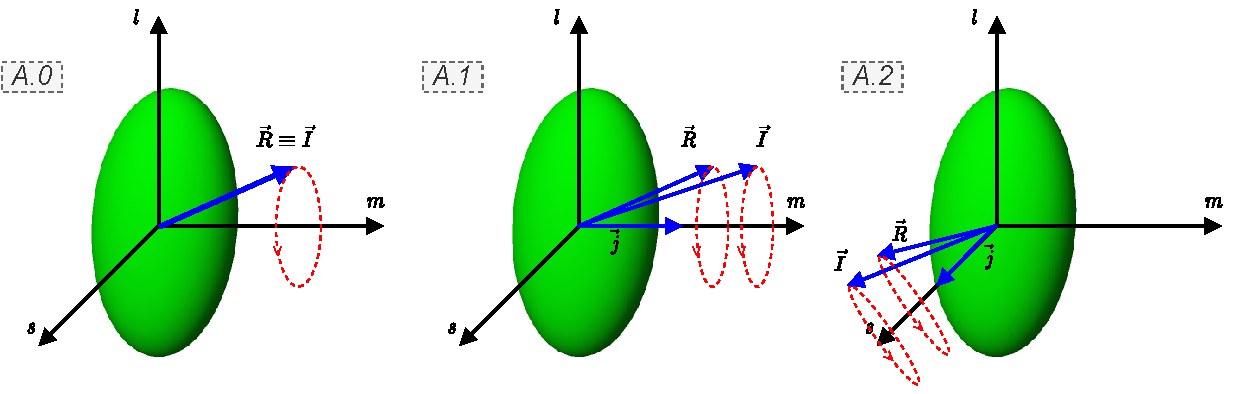
\includegraphics[width=0.9\textwidth]{figs/wobbling_Regimes_COUPLING_SCHEME.pdf}
    \caption{A.0: The geometry for the angular momentum of a simple wobbler. A.1: coupling geometry for a longitudinal wobbler (LW). A.2: coupling geometry for a transverse wobbler (TW). The short-$s$, long-$l$, and medium-$m$ axes are defined in the body-fixed frame. The vectors $\vec{R}$, $\vec{j}$, and $\vec{I}$ represent the set of angular momenta of the core, odd particle, and the total nuclear system, respectively.}
    \label{wobbling-coupling-scheme}
\end{figure}

\section{A new formalism for the descritpion of wobbling states}
In this section, a discussion on the latest work regarding the wobbling properties in an odd-mass nucleus will be made.

\begin{figure}
    \centering
    % 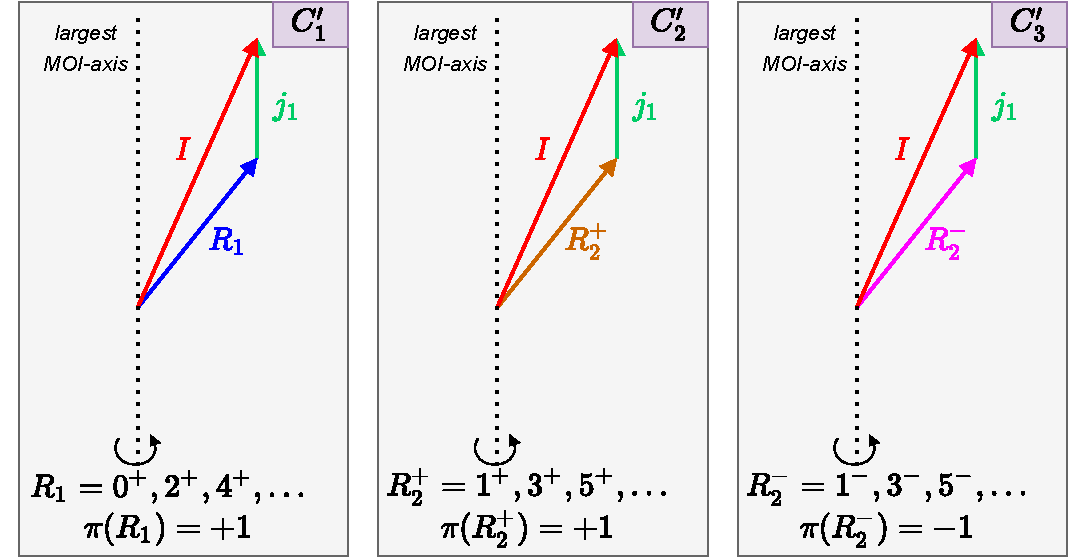
\includegraphics[width=0.95\textwidth]{figs/coupling_schemes_C1C2C3.pdf}
    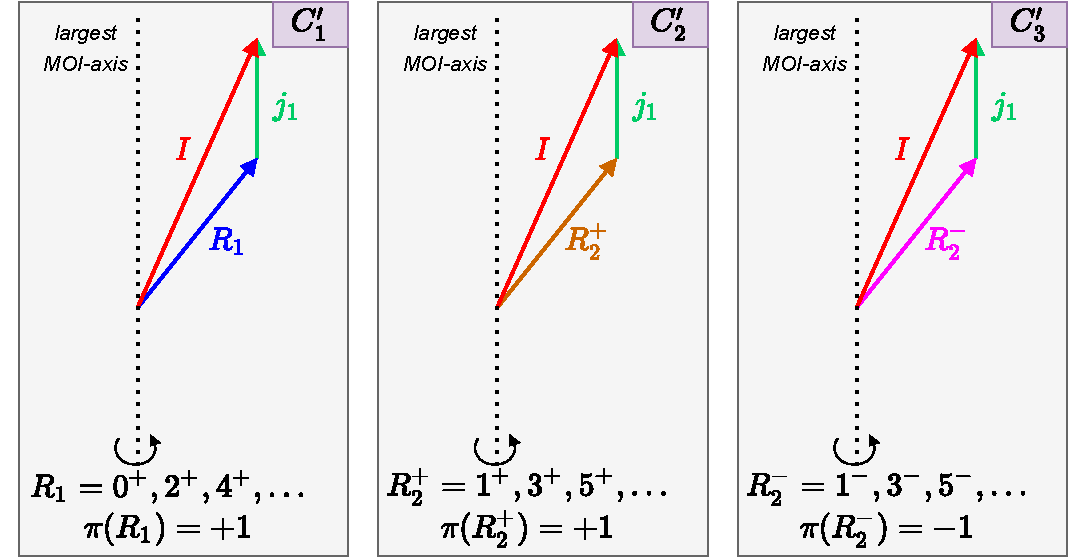
\includegraphics[scale=0.7]{figs/coupling_schemes_C1C2C3.pdf}
    \caption{A schematic representation with the three coupling schemes that characterize the \texttt{W2} model. The same odd particle ($j_1=i_{13/2}$ proton) is coupled with two positive cores with even (odd) integer spin sequences for $TSD_1$ ($TSD_2$), and one negative core in the case of $TSD_4$ with odd integer spin sequence. The total spin of the system precesses around the axis with the largest MOI, as it is the case for a triaxial rotor.}
    \label{three-couplings}
\end{figure}

Similar structures with alternating positive-negative parity bands have been also reported in other nuclei such as $^{40}$Ca \cite{torilov2004spectroscopy}, or some heavier isotopes like $^{218}$Fr \cite{debray2000alternating}. In fact, a unified description of states with positive and negative parity in odd-mass nuclei was made over the last decade \cite{radutaa2009csm,raduta2011simultaneous}, although therein, a quadrupole-octupole term was introduced within the particle-core Hamiltonian to describe this feature. A diagram which shows the workflow involved in \texttt{W2} can be seen in the Figure \ref{w2-model-worfklow} from the Appendix \ref{appendix:a}.


\section{Theoretical Formalism}
\label{section-theory}

In this section, a description of the framework used for obtaining the wobbling spectrum of $^{163}$Lu is made. As stated in the previous section, the system is described with a similar Hamiltonian used in \texttt{W1}, namely the Hamiltonian for the triaxial PRM.
\begin{align}
    H=H_\text{core}+H_\text{s.p.}\ .
    \label{prm-hamiltonian}
\end{align}

The Hamiltonian from Eq. \ref{prm-hamiltonian} describes a system in which an odd $j$ particle interacts with a triaxial even-even core i.e., the odd nucleon is moving in a quadrupole deformed mean-field that is generated by the core. As such, the first term in the Hamiltonian $H_\text{core}$ describes the motion of a triaxial core, while the second term $H_\text{s.p.}$ represents the single-particle potential characterizing the valence proton.

Indeed, the core Hamiltonian is given by:
\begin{align}
    H_\text{core}=\sum_{i=1,2,3}\frac{1}{2\mathcal{I}_i}(I_i-j_i)^2\ ,
    \label{core-hamiltonian}
\end{align}
where the core angular momentum is $\vec{R}=\vec{I}-\vec{j}$ and the terms $\mathcal{I}_i$ represent the moments of inertia for a triaxial ellipsoid, along the principal axes. These three moments of inertia will be considered as free parameters in the present calculations, but, compared to the work \texttt{W1}, a unique set of MOIs will be attributed to the four bands, since the triaxial core will create an alignment with a unique particle, that is $j_1$. Because of this, there is no option for their nature (i.e., rigid or hydrodynamic).

The single-particle Hamiltonian from Eq. \ref{prm-hamiltonian} is derived from the well-known Nilsson potential \cite{meyer1975collective,wang2008description}:
\begin{align}
    h(\beta_2,\gamma)=C\left\{\cos\gamma Y_{20}(\theta,\varphi)+\frac{\sin\gamma}{\sqrt{2}}\left[Y_{22}(\theta,\varphi)+Y_{2-2}(\theta,\varphi)\right]\right\}\ ,
    \label{nilsson-potential}
\end{align}
where the coupling parameter $C$ causes the level splitting in the deformed field and it is proportional to the quadrupole deformation $\beta_2$. The potential $h$ from Eq. \ref{nilsson-potential} is written in terms of the quadrupole deformation and triaxiality parameter that play the role of deformation parameters within a triaxial system $(\beta_2,\gamma)$. Its expression using the coupling parameter $C$ is widely used when working with a particle-rotor-model \cite{peng2003description,koike2004chiral,wang2007doublet}. In the present this case, the change $h(\beta_2,\gamma)\to H_\text{s.p.}$ is done by applying the Wigner-Eckart theorem for the single-$j$ particle, and the following expression for $H_\text{s.p.}$ will be obtained:
\begin{align}
    H_\text{s.p.}=\frac{V}{j(j+1)}\left[\cos\gamma(3j_3^2-\vec{j}^2)-\sqrt{3}\sin\gamma(j_1^2-j_2^2)\right]+\epsilon_j\ .
    \label{single-particle-hamiltonian}
\end{align}

This term describes the motion of an odd particle with angular momentum $j$ in a mean-field generated by a triaxial core, with a potential strength $V$ characterized by the quadrupole deformation ($V\propto\beta_2)$. In fact, the single-particle potential strength $V$ will be considered as the fourth free parameter within the calculations and its behavior will dictate the coupling of the $j$ particle with all four TSD bands. The term $\epsilon_j$ from Eq. \ref{single-particle-hamiltonian} represents the single-particle energy that corresponds to the odd $j$ proton from the $i$-orbital. One should not mix up the $j_1$ proton notation used throughout the paper with the components of the single-particle angular momentum from  Eq. \ref{single-particle-hamiltonian}.

Regarding the triaxial deformation $\gamma$ which enters in Eq. \ref{single-particle-hamiltonian}, its value will be considered as another free parameter of the current problem. In other words, having $V$ and $\gamma$ as free parameters means that the system will be described by its deformation parameters which will be obtained through a fitting procedure, keeping an agreement with the experimental data regarding the excitation energies of the rotational states belonging to $TSD_{1,2,3,4}$.

From Eqs. \ref{core-hamiltonian} and \ref{single-particle-hamiltonian}, the free parameter set can be obtained, hereafter denoted by $\mathcal{P}$. It comprises three moments of inertia, the single-particle potential strength, and the triaxial deformation. As such, $\mathcal{P}$ can be written as:
\begin{align}
    \mathcal{P}=\left[\mathcal{I}_1,\mathcal{I}_2,\mathcal{I}_3,V,\gamma\right]\ .
    \label{parameter-set}
\end{align}

Solving the problem of \texttt{W2} is equivalent to finding the eigenvalues of $H$ given in Eq. \ref{prm-hamiltonian}. In a similar approach as in \texttt{W1}, the eigenvalues of interest are obtained on the base of a semi-classical approach. Thus, the first step is to perform a de-quantization procedure on $H$ through a TDVE \cite{raduta2007semiclassical,budaca2018tilted,raduta2017semiclassical}:
\begin{align}
    \delta\int_0^t\bra{\Psi_{IjM}}H-i\frac{\partial}{\partial t'}\ket{\Psi_{IjM}}dt'=0\ .
    \label{tdve}
\end{align}

Working within a semi-classical approach allows one to keep close contact with the system's dynamics in terms of equations of motion for the generalized coordinates. The trial function from Eq. \ref{tdve} is carefully chosen as a product of two basis states comprising the states with total angular momentum $I$ and $j$, respectively:
\begin{align}
    \ket{\Psi_{IjM}}=\mathbf{N}e^{z\hat{I}_-}e^{s\hat{j}_-}\ket{IMI}\ket{jj}\ ,
    \label{trial-function}
\end{align}
where the operators $\hat{I}_-$ and $\hat{j}_-$ denote the lowering operators for the intrinsic angular momenta $\vec{I}$ and $\vec{j}$, respectively, and $\mathbf{N}$ plays the role of the normalization constant. One must remark the fact that the states $\ket{IMI}$ and $\ket{jj}$ from Eq. \ref{trial-function} are extremal states for the operators $(\hat{I}^2,\hat{I}_3)$ and $(\hat{j^2},\hat{j_3})$, respectively, and they correspond to the maximally allowed states for a given set of angular momenta $I$ and $j$. As an observation, the trial function is an admixture of components of definite $K$, which is consistent with the fact that for a triaxial nucleus, $K$ is not a good quantum number.

The variables $z$ and $s$ from Eq. \ref{trial-function} are complex functions of time, and they play the role of classical coordinates in the phase spaces that describe the motion of the core and the odd particle:
\begin{align}
    z=\rho e^{i\varphi}\ ,\ s=fe^{i\psi}\ .
    \label{complex-variable-set}
\end{align}

In order to obtain a set of classical equations in a Hamilton Canonical form, a new pair of variables are introduced: 
\begin{align}
    r=\frac{2I}{1+\rho^2}\ ,\ t=\frac{2j}{1+f^2}\ ,
\end{align}
where $r\in\left[0,2I\right]$ and $t\in\left[0,2j\right]$.Thus the equations of motion acquire the form:
\begin{align}
    \frac{\partial\mathcal{H}}{\partial r}&=\dot{\varphi}\ ;\ \frac{\partial\mathcal{H}}{\partial \varphi}=-\dot{r}\ , \nonumber\\
    \frac{\partial\mathcal{H}}{\partial t}&=\dot{\psi}\ ;\ \frac{\partial\mathcal{H}}{\partial \psi}=-\dot{t}\ .
    \label{eq-motion}
\end{align}

The function $\mathcal{H}$ denotes the average of the Hamiltonian operator $H$ (Eq. \ref{prm-hamiltonian}) with the trial function $\ket{\Psi_{IjM}}$ given in Eq. \ref{trial-function}, and it plays the role of classical energy:
\begin{align}
    \mathcal{H}(\varphi,r;\psi,t)=\bra{\Psi_{IjM}}H\ket{\Psi_{IjM}}\ ,
\end{align}

Starting from the equations of motion given in Eq. \ref{eq-motion}, one can observe that the function $\mathcal{H}$ is a constant of motion, that is $\dot{\mathcal{H}}\equiv0$. This equation will define a surface, a so-called equi-energy surface $\mathcal{H}=\text{const}$. It is worth mentioning the fact that such equality holds since the entire set of equations of motion emerged from a variational principle. The sign of the Hessian associated to this classical function will indicate its stationary points. Among them, some are minima. The critical points which are of interest for the present study are those obtained when the following ordering for the three moments of inertia holds: $\mathcal{I}_1>\mathcal{I}_2>\mathcal{I}_3$. There is no restriction on $\gamma$.

With a linearization procedure for the equations of motion around the minimum point  of $\mathcal{H}$, a dispersion equation will be obtained:
\begin{align}
    \Omega^4+B\Omega^2+C=0\ .
    \label{dispersion-eq}
\end{align}

The above equation describes a harmonic type of motion for the nuclear system, with the solutions to this algebraic equation as the \emph{wobbling frequencies} $\Omega$. The terms $B$ and $C$ are  functions of total angular momentum $I$, single-particle a.m. $j$, inertial parameters $A_k=1/(2\mathcal{I}_k)\ ,\ k=1,2,3$, single-particle potential strength $V$, and triaxiality parameter $\gamma$.  The $B$ term from Eq. \ref{dispersion-eq} has the expression \cite{raduta2020approach}:
\begin{align}
 -B=\left[(2I-1)(A_3-A_1)+2jA_1\right]\left[(2I-1)(A_2-A_1)+2jA_1\right]+8A_2A_3Ij+\text{T}_B^1\text{T}_B^2\ ,
 \label{b_term}
 \end{align}
 where the terms $\text{T}_B^1$ and $\text{T}_B^2$ are defined defined as:
 \begin{align}
 \text{T}_B^1&=\left[(2j-1)(A_3-A_1)+2IA_1+V\frac{2j-1}{j(j+1)}\sqrt{3}(\sqrt{3}\cos\gamma+\sin\gamma)\right]\ , \nonumber \\
 \text{T}_B^2&=\left[(2j-1)(A_2-A_1)+2IA_1+V\frac{2j-1}{j(j+1)}2\sqrt{3}\sin\gamma\right]\ .
 \label{b_term-plus}
\end{align}

Accordingly, the $C$ term from Eq. \ref{dispersion-eq} has the expression \cite{raduta2020approach}:
\begin{align}
    C=&\left\{\left[(2I-1)(A_3-A_1)+2jA_1\right]\text{T}_C^1
- 4IjA_3^2\right \} \nonumber\\
      &\times\left\{\left[(2I-1)(A_2-A_1)+2jA_1\right]\text{T}_C^2-4IjA_2^2\right\}\ ,
      \label{c_term}
\end{align}
where the terms $\text{T}_C^1$ and $\text{T}_C^2$ are defined defined as:
\begin{align}
    \text{T}_C^1&=\left[(2j-1)(A_3-A_1)+2IA_1+V\frac{2j-1}{j(j+1)}\sqrt{3}(\sqrt{3}\cos\gamma+\sin\gamma)\right]\ , \nonumber\\
    \text{T}_C^2&=\left[(2j-1)(A_2-A_1)+2IA_1+V\frac{2j-1}{j(j+1)}2\sqrt{3}\sin\gamma\right]\ . 
    \label{c_term-plus}
\end{align}

It can be seen that the terms which enter in $B$ and $C$, namely $(\text{T}_B^1,\text{T}_B^2)$ from Eq. \ref{b_term-plus} and $(\text{T}_C^1,\text{T}_C^2)$ from Eq. \ref{c_term-plus} correspond to the quadrupole deformation that causes the single-particle to move in the mean-field of the triaxial core. The terms also define the triaxiality that the nucleus achieves once the odd proton couples to the triaxial core, driving the system up to a large (and stable) deformation.

Going back to Eq. \ref{dispersion-eq}, under the restrictions for the MOIs defined above, the dispersion equation admits two real and positive solutions (hereafter denoted with $\Omega_1^I$ and $\Omega_2^I$, where $\Omega_1^I<\Omega_2^I$) defined for $j_1=i_{13/2}$, given by:
\begin{align}
    \Omega_{1,2}^I=\sqrt{\frac{1}{2}\left(-B\mp(B^2-4C)^{1/2}\right)}\ .
    \label{wobbling-frequencies}
\end{align}

These two solutions are interpreted as \emph{wobbling frequencies} associated with the motion of the core, and the motion of the odd-particle respectively. As such, each wobbling frequency has an associated wobbling-phonon number:
\begin{align}
    \Omega_1^I \to n_{w_1}\ ;\ \Omega_2^I \to n_{w_2}\ .
\end{align}


Now  the analytical expressions for the four TSD bands in $^{163}$Lu are readily obtained:
\begin{align}
    E_\text{TSD1}^I&=\epsilon_j+\mathcal{H}_\text{min}^{(I,j)}+\mathcal{F}_{00}^I\ ,\ I=13/2,17/2,21/2\dots \nonumber \\
    E_\text{TSD2}^I&=\epsilon_j^1+\mathcal{H}_\text{min}^{(I,j)}+\mathcal{F}_{00}^I\ ,\ I=27/2,31/2,35/2\dots \nonumber \\
    E_\text{TSD3}^I&=\epsilon_j+\mathcal{H}_\text{min}^{(I-1,j)}+\mathcal{F}_{10}^{I-1}\ ,\ I=33/2,37/2,41/2\dots \nonumber \\
    E_\text{TSD4}^I&=\epsilon_j^2+\mathcal{H}_\text{min}^{(I,j)}+\mathcal{F}_{00}^I\ ,\ I=47/2,51/2,55/2\dots\ ,
    \label{wobbling_energies}
\end{align}
where $\mathcal{F}_{n_{w_1}n_{w_2}}^I$ is a function of the wobbling frequencies:
\begin{align}
    \mathcal{F}_{n_{w_1}n_{w_2}}^I=\Omega_1^I\left(n_{w_1}+\frac{1}{2}\right)+\Omega_2^I\left(n_{w_2}+\frac{1}{2}\right)\ ,
    \label{f-term}
\end{align}
and $\mathcal{H}_\text{min}^{(I,j)}$ is the classical energy evaluated in its minimal point. For the present case, its analytical expression is given by the following equation:
\begin{align}
\mathcal{H}_\text{min}^{(I,j)}=(A_2+A_3)\frac{I+j}{2}+A_1(I-j)^2-V\frac{2j-1}{j+1}\sin\left(\gamma+\frac{\pi}{6}\right)\ .
    \label{hmin:equation}
\end{align}

A few aspects regarding the energy spectrum defined in Eq. \ref{wobbling_energies} are worth mentioning. To each band, there is a specific energy $\epsilon_j$ associated with the single-particle state. In this case, the odd-proton $j_1=13/2$ from the $i$-orbital is the one that couples to the triaxial core. However, for the bands $TSD_2$ and $TSD_4$, a different re-normalization of $\epsilon_j$ is considered, since $TSD_2$ is the unfavored signature partner of $TSD_1$, and $TSD_4$ is the negative parity partner of $TSD_2$ within the band structure. These quantities will shift the overall energy states belonging to the two bands, each by a different amount. As a result, both $\epsilon_j^1$ and $\epsilon_j^2$ will be adjusted throughout the numerical calculations such that the energy spectrum is best reproduced. Another aspect concerns the band $TSD_3$; since this is the only excited wobbling band within the family, its configuration is built on top of $TSD_2$, with the action of a single phonon ($n_{w_1}=1$) operator. Consequently, an energy state $I$ belonging to $TSD_3$ is obtained from a state $I-1$ from $TSD_2$. In Table \ref{energy-states-tabular}, the rest of the wobbling phonon numbers are mentioned, with the parity, signature, and coupling scheme for each band in particular.

\begin{table}
\centering
\begin{tabular}{llllll}
\hline
Band & $n_{w_1}$ & $n_{w_2}$ & $\pi$ & $\alpha$ & Coupling scheme\\
\hline
\hline
   $TSD_1$  &   0        &    0       & +1      &    +1/2      &   $C'_1$              \\
   $TSD_2$  &     0      &      0     &   +1    &  -1/2        &   $C'_2$              \\
   $TSD_3$  &   1        &      0     &     +1  &     +1/2    &  Built on top of $TSD_2$                \\
   $TSD_4$  &    0       &      0     &      -1 &   -1/2       &    $C'_3$    \\       
   \hline
\end{tabular}
\caption{The wobbling phonon numbers, parities, signatures, and coupling schemes assigned to each triaxial band in $^{163}$Lu, within the \texttt{W2} model. The three coupling schemes were defined in Section \ref{subsection:w2}.}
\label{energy-states-tabular}
\end{table}

\subsection{Parity quantum number for the wave-function}

In \texttt{W1} it was shown that signature emerges from the calculations on the total wave-function as a good quantum number for this triaxial system. This is why in \cite{raduta2020approach} the bands $TSD_1$ and $TSD_2$ appeared as Signature Partner Bands (SPB). In \texttt{W2}, such property still stands.

Since the backbone of the current work started from the need for a single odd-particle that couples to a triaxial core in $^{163}$Lu, one has to look at the band $TSD_4$ (which was interpreted as having a different nucleon: $j_2$ with $j=9/2$ from the $h$-orbital), and see if its differentiating properties can be linked to \emph{main group} of bands (namely $TSD_{1,2,3}$). Indeed, from the experimental measurements regarding spin and parity assignment \cite{jensen2004coexisting}, it turns out that the parity of the rotational states is negative. Therefore, a forensic analysis on this quantum property should be considered as the necessary ingredient in a unified description of all four bands.

 The parity operator is defined as a product of the complex conjugation operation and a rotation of angle $\pi$ around the 2-axis: $P=e^{-i\pi\hat{I}_2}C$. The total parity operator is the product of an operator corresponding to the core and one corresponding to the single-particle:
\begin{align}
    \mathcal{P}_T=P_\text{core}P_\text{s.p.}\ .
    \label{parity-operator}
\end{align}

Acting with the total parity operator defined above, on the trial function $\Psi$ associated , the following result is obtained:
\begin{align}
    \mathcal{P}_T\Psi(r,\varphi;t,\psi)=\Psi(r,\varphi+\pi;t,\psi+\pi)\overset{\mathrm{not.}}{=}\ \bar{\Psi}.
    \label{parity-action}
\end{align}

The classical energy function $\mathcal{H}$ has an invariance property at changing the angles with $\pi$:
\begin{align}
    \mathcal{H}(r,\varphi;t,\psi)=\mathcal{H}(r,\varphi+\pi;t,\psi+\pi)\ .
    \label{classical-energy-invariance}
\end{align}

From Eqs. \ref{parity-action} and \ref{classical-energy-invariance}, it can be concluded that the wave-function describing the triaxial system $\Psi$ and its image through $\mathcal{P}_T$ , $\bar{\Psi}$,  are two linearly dependent functions which differ only by a multiplicative constant $p$, with $|p|=1$. Thus, $p$ can either be -1 or +1, such that:
\begin{align}
    % \Psi(r,\varphi+\pi;t,\psi+\pi)=\pm\Psi(r,\varphi;t,\psi)\ .
    \bar{\Psi}=\pm\Psi(r,\varphi;t,\psi)\ .
\end{align}

The above result concludes the parity analysis for the wave-function, showing that the triaxial rotor admits eigenfunctions of negative parity. Therefore, a single wave-function characterized by the coupling of a triaxial core to the odd proton $i_{13/2}$ is describing both positive parity states ($\in TSD_{1,2,3}$) as well as negative parity states ($\in TSD_4$). This analysis, together with the fact that $TSD_2$ and $TSD_4$ have the same a.m. sequences (although $TSD_2$ has more states with low spin than $TSD_4$) suggest the fact that these two bands might be Parity Partners.

\subsection{Energy function - geometrical interpretation}

The analytical expression for the average of $H$ with the trial function describing the system was previously calculated in \texttt{W1}. Indeed, the energy function $\mathcal{H}$ was given in terms of the phase space coordinates $(r,\varphi;t,\psi)$ as follows \cite{raduta2020approach}:
\begin{align}
    \mathcal{H}=&\frac{I}{2}(A_1+A_2)+A_3I^2+\frac{2I-1}{2I}r(2I-r)\mathcal{A}_\varphi+\frac{j}{2}(A_1+A_2)+A_3j^2+\frac{2j-1}{2j}t(2j-t)\mathcal{A}_\psi \nonumber\\
    &-2\sqrt{r(2I-r)t(2j-t)}\mathcal{A}_{\varphi\psi}+A_3\left[r(2j-t)+t(2I-r)\right]-2A_3Ij+V\frac{2j-1}{j+1}\mathcal{A}_\gamma\ ,
    \label{energy-function-analytical}
\end{align}
with:
\begin{align}
    &\mathcal{A}_\varphi(\varphi)=(A_1\cos^2\varphi+A_2\sin^2\varphi-A_3)\ , \nonumber\\
    &\mathcal{A}_{\varphi\psi}(\varphi,\psi)=(A_1\cos\varphi\cos\psi+A_2\sin\varphi\sin\psi)\ ,\nonumber\\
    &\mathcal{A}_\psi(\psi)=(A_1\cos^2\psi+A_2\sin^2\psi-A_3)\ , \nonumber\\
    &\mathcal{A}_\gamma(t,\psi)=\left[\cos\gamma-\frac{t(2j-t)}{2j^2}\sqrt{3}(\sqrt{3}\cos\gamma+\sin\gamma\cos2\psi)\right]\ .
\end{align}

It is instructive to check the dependence of the energy function on the angular momentum components, e.g., the coordinates $x_k\overset{\mathrm{not.}}{=}I_k\ ,\ k=1,2,3$, where the quantization axis is chosen as the 3-axis. By expressing the angular momentum coordinates $x_{1,2,3}$ in terms of the polar angles $(\theta,\varphi)$ and a radius $I$ , one obtains: 
\begin{align}
    x_1=I\sin\theta\cos\varphi\ ,\ x_2=I\sin\theta\sin\varphi\ ,\ x_3=I\cos\theta\ .
    \label{coordinate-parametrization}
\end{align}

Within this spherical coordinates, and evaluating the energy function around its minimum point $p_0=(0,I;0,j)$, the following expression for $\mathcal{H}$ results:
\begin{align}
    \left. \mathcal{H}\ \right\vert_{p_0}=I\left(I-\frac{1}{2}\right)\sin^2\theta(A_1\cos^2\varphi+A_2\sin^2\varphi-A_3)-2A_1Ij\sin\theta+T_\text{core}+T_\text{s.p.}\ .
    \label{energy-function-minimal}
\end{align}

The last two terms in this equation are independent on the polar angles $(\theta,\varphi)$, and  have the form:
\begin{align}
    T_\text{core}&=\frac{I}{2}(A_1+A_2)+A_3I^2\ ,\nonumber \\
    T_\text{s.p.}&=\frac{j}{2}(A_2+A_3)+A_1j^2-V\frac{2j-1}{j+1}\sin\left(\gamma+\frac{\pi}{6}\right)\ .
    \label{energyfunction-core-single-particle-subterms}
\end{align}

The classical equations of motion admit two constants of motion: the total energy (E) and the total angular momentum (I).  Consequently, by finding the intersection line(s) between the surface of the energy ellipsoid $E$ and the surface of the angular momentum, a sphere of radius  $I$, one finds the system trajectory.  Such representations will be made in the following section.

The expression of the energy ellipsoid in Cartesian coordinates is:
\begin{align}
    E=&\left(1-\frac{1}{2I}\right)A_1x_1^2+\left(1-\frac{1}{2I}\right)A_2x_2^2+\left[\left(1-\frac{1}{2I}\right)A_3+A_1\frac{j}{I}\right]x_3^2-\nonumber\\
    &-I\left(I-\frac{1}{2}\right)A_3-2A_1Ij+T_\text{rot}+T_\text{sp}\ .
    \label{energy-ellipsoid-cartesian}
\end{align}

 For a total angular momentum $\vec{I}$, the vector generates a sphere of radius $r=I$ described by the equation:
\begin{align}
    I^2=x_1^2+x_2^2+x_3^2\ .
    \label{angular-momentum-sphere}
\end{align}

The trajectories obtained through the intersection of Eqs. \ref{energy-ellipsoid-cartesian} and \ref{angular-momentum-sphere} will show a classical visualization of the wobbling character for a triaxial nucleus.

\section{Numerical results}
\label{section-results}

As a first step, the results concerning the excited spectrum of the four TSD bands will be presented. Regarding the wobbling spectrum of $^{163}$Lu, its analytical formulation was given in Eq. \ref{wobbling_energies}. As mentioned, those energies are parametrized in terms of $\mathcal{P}$, which is the set of free parameters to be determined. Indeed, one can find $\mathcal{P}$ by minimizing the $\chi^2$ function:
\begin{align}
    \chi^2=\frac{1}{N_T}\sum_{i}\frac{(E^{(i)}_\text{exp}-E^{(i)}_\text{th})^2}{E^{(i)}_\text{exp}}\ ,
    \label{chi-square}
\end{align}
where $N_T$ represents the total number of states. Table \ref{4-band-information} contains the number of states within each band, with the spin sequences for the core ($\vec{R}$), the spin sequences for the coupled system (that is the total angular momentum $\vec{I})$, and the coupling schemes specific to \texttt{W2} formalism that is used in the current calculations. 

\begin{table}
    \centering
  \begin{tabular}{llllll}
  \hline
  Band & $n_s$ & $\vec{j}$ & $\vec{R}$ - Sequence & $\vec{I}$ - Sequence & Coupling scheme \\
  \hline
  \hline
     $TSD_1$ &       21      &   $j_1$  &        $R_1=0,2,4,\dots$         &   $13/2,17/2,21/2,\dots$    & $C'_1$     \\
     $TSD_2$ &        17     &   $j_1$   &       $R_2^+=1^+,3^+,5^+,\dots$             &      $27/2,31/2,35/2,\dots$                &      $C'_2$           \\
     $TSD_3$ &      14       &    $j_1$  &           1-phonon excitation         & $33/2,37/2,41/2,\dots$                &       1-phonon excitation           \\
     $TSD_4$ &       11      &   $j_1$   &    $R_2^-=1^-,3^-,5^-,\dots$                &               $47/2,51/2,55/2,\dots$         &      $C'_3$          \\
     \hline
\end{tabular}
    \caption{The number of energy states $n_s$ within each wobbling band, the a.m. of the proton $\vec{j}$, the core's a.m. $\vec{R}$, the nucleus' a.m. $\vec{I}$, and the corresponding coupling scheme that was established according to the \texttt{W2} model. The single-particle is the $j_1=(i_{13/2})$ proton.}
    \label{4-band-information}
\end{table}

The resulting values for $\mathcal{P}$ are given  in Table \ref{parameter_set}. This \texttt{W2} method contrasts the approach in \texttt{W1}, where a second minimization process was needed separately for $TSD_4$. The root mean square error provided by the obtained parameter set $\mathcal{P}$ has a value of $E_\text{rms}\approx 79\ \text{keV}$. This result is much better than the one obtained with previous formalism \texttt{W1} where an $E_\text{rms}\approx240\ \text{keV}$ was obtained \cite{raduta2020approach}). As a matter of fact, this is the first semi-classical formalism in the literature that achieves agreement with the experimental data with less than $100\ \text{keV}$ for the entire wobbling spectrum of $^{163}$Lu. It is worth mentioning that the fitting procedure was done not for the absolute wobbling energies $E_\text{TSDk}^I\ ,\ k=1,2,3,4$, but for the \emph{excitation energies} which are relative to the hand-head $I=13/2^+$ from the first yrast band $TSD_1$. Comparison between the theoretical values obtained within the current formalism and the experimental data is shown in Figures \ref{energies-tsd12} and \ref{energies-tsd34}. For the sake of completeness, the wobbling frequencies which enter in the expression of the $\mathcal{F}_{n_{w_1}n_{w_2}}^I$ given by Eq. \ref{f-term} are graphically represented as functions of total angular momentum $I$ in Figure \ref{hydro-mois}, for the fixed parameter set. It is remarkable the fact that the wobbling frequency $\Omega_2^I$ is much larger than its partner, suggesting the fact the coupling effects caused by the highly aligned proton have a stronger influence in achieving a wobbling character for $^{163}$Lu, which is in line with the characteristics of a particle-rotor coupling. Another feature of these wobbling frequencies is their linear behavior with respect to the nuclear spin.

\begin{table}
    \centering
  \begin{tabular}{lllll}
  \hline
$\mathcal{I}_1$ [$\hbar^2$/\text{MeV}] & $\mathcal{I}_2$ [$\hbar^2$/\text{MeV}]& $\mathcal{I}_3$ [$\hbar^2$/\text{MeV}] & $\gamma$ [deg. ] & $V$ [\text{MeV}] \\
\hline
\hline
72              & 15              & 7               & 22       & 2.1\\
\hline
\end{tabular}
    \caption{The parameter set $\mathcal{P}$ that was determined by a fitting procedure of the excitation energies for $^{163}$Lu. }
    \label{parameter_set}
\end{table}

Concerning the single-particle energies from Eq. \ref{wobbling_energies}, namely $\epsilon_j^1$ and $\epsilon_j^2$ that emerge from the un-favored signature of $TSD_2$ and negative parity of $TSD_4$, respectively, they induce a correction for the mean-field with the quantities $\epsilon_j^1-\epsilon_j=0.3\ \text{MeV}$ and $\epsilon_j^2-\epsilon_j=0.6\ \text{MeV}$. Note that since the energy state $I_{13/2}\in TSD_1$ (the band-head of $TSD_1$) was subtracted from all bands, the single-particle energies for band 2 and 4 are adjusted accordingly.

The quantity $\epsilon_j^1-e_j$ is added to the second band due to the core, and such a splitting is caused by the fact that two distinct TDVE procedures were performed for the two partner bands $TSD_{1,2}$. The total signature splitting for the band-head and the terminus states of $TSD_2$ are $E_{TSD2}^{27/2}-E_{TSD2}^{25/2}=0.492\ \text{MeV}$ and $E_{TSD2}^{91/2}-E_{TSD2}^{89/2}=0.936\ \text{MeV}$ which agrees with the estimate made by Jensen et. al. in \cite{jensen2002wobbling}. Although the signature splitting can be determined microscopically by using a deformed single-particle basis amended with a cranking constraint, for the present case it is obtained by applying the TDVE for each spin state and the correction corresponding to the single-particle energies (that is $\epsilon_j^1$).

\begin{figure}
\centering
\begin{minipage}{.5\textwidth}
  \centering
  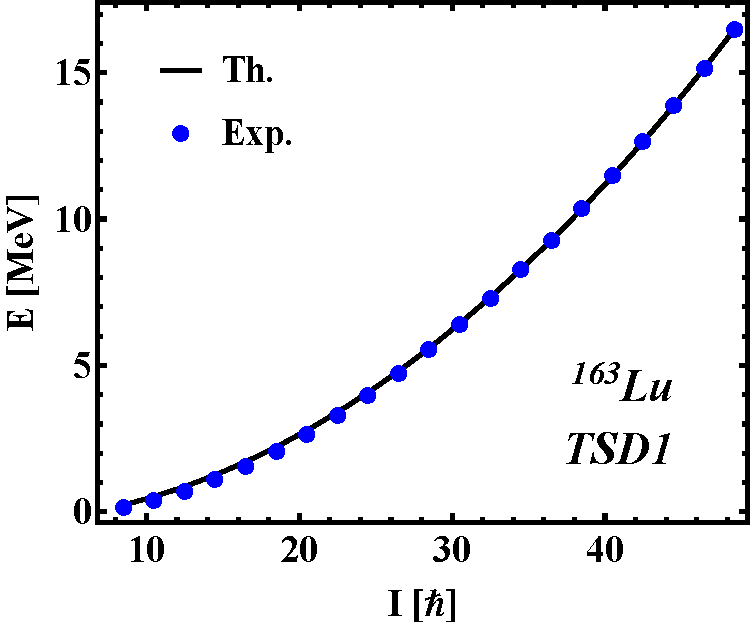
\includegraphics[scale=0.55]{figs/DoubleShift_TSD1.pdf}
\end{minipage}%
\begin{minipage}{.5\textwidth}
  \centering
 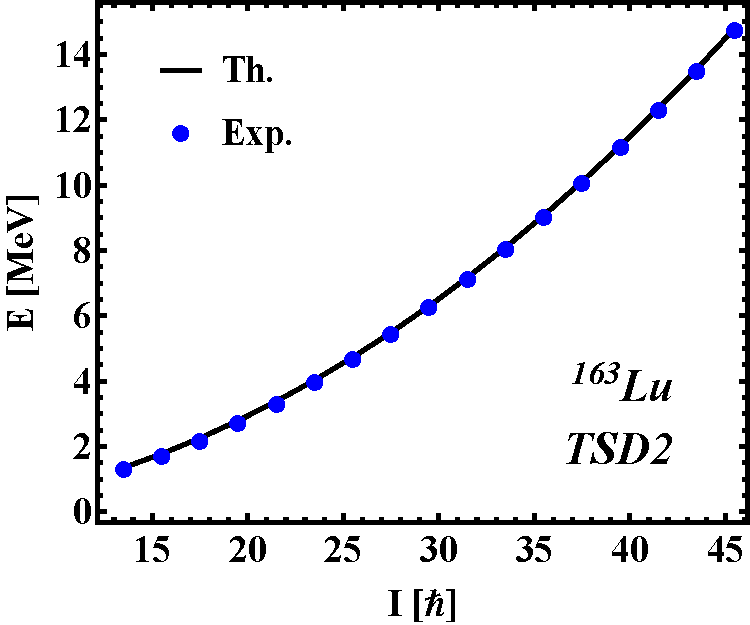
\includegraphics[scale=0.55]{figs/DoubleShift_TSD2.pdf}
\end{minipage}
\caption{Comparison between theoretical and experimental excitation energies for the first two wobbling bands in $^{163}$Lu within the \texttt{W2} model. The theoretical results are obtained with the parameters listed in Table \ref{parameter_set}. Experimental data is taken from \cite{reich2010nuclear}.}
\label{energies-tsd12}
\end{figure}

\begin{figure}
\centering
\begin{minipage}{.5\textwidth}
  \centering
  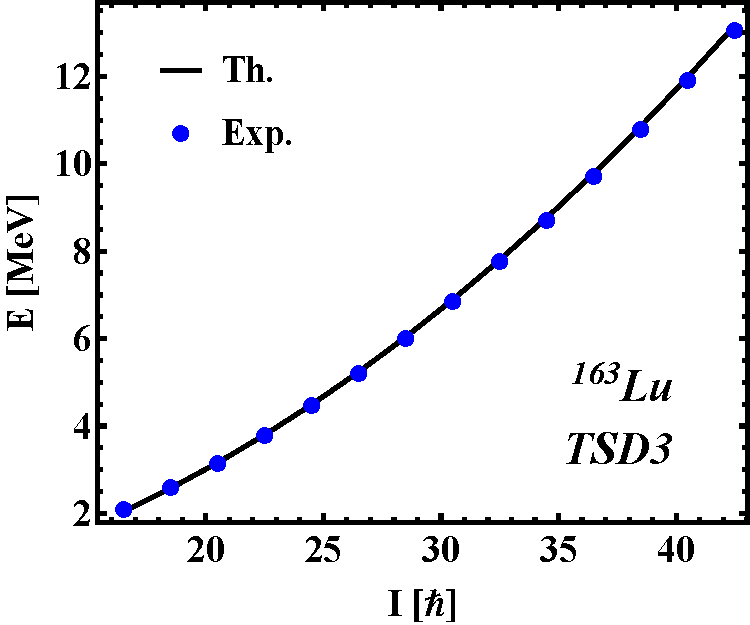
\includegraphics[scale=0.55]{figs/DoubleShift_TSD3.pdf}
\end{minipage}%
\begin{minipage}{.5\textwidth}
  \centering
 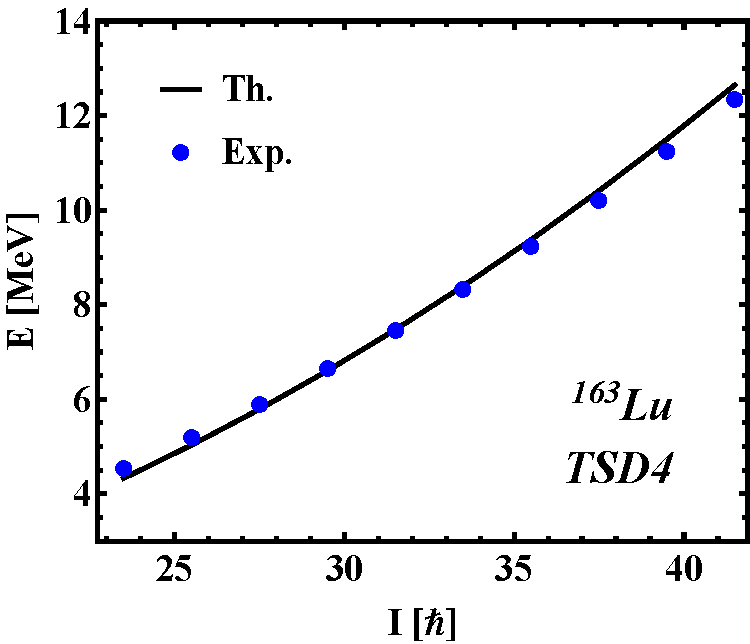
\includegraphics[scale=0.55]{figs/DoubleShift_TSD4.pdf}
\end{minipage}
\caption{Comparison between theoretical and experimental excitation energies for third and fourth wobbling bands in $^{163}$Lu within the \texttt{W2} model. The theoretical results are obtained with the parameters listed in Table \ref{parameter_set}. Experimental data is taken from \cite{reich2010nuclear}.}
    \label{energies-tsd34}
\end{figure}

Another noteworthy aspect of the current formalism is the fact that the difference $\delta_{42}=E_\text{TSD4}^I-E_\text{TSD2}^I$ for all the states has an almost constant value $\delta_{42}\approx0.3\ \text{MeV}$. This suggests that the states of the same a.m. from $TSD_2$ and $TSD_4$ bands might emerge through the parity projection of a sole wave-function that does not have reflection symmetry. In the present case, this is caused by the fact that the wobbling frequency is parity-independent. It is interesting that the action of the parity operator on any rotational state within the angular momentum space will lead to the change of the angular momentum vector from $\vec{I}$ to $-\vec{I}$. Due to this reason, the parity operator commutes with the initial Hamiltonian, and the eigenfunctions of $H$ are characterized by either positive or negative parity (with states of different parities being degenerate). However, one can lift this degeneracy by using an additional linear in the expression $H$. Since in Eq. \ref{prm-hamiltonian} such a linear term is missing, an \emph{ad-hoc} correction of the mean-field with the amount $0.6\ \text{MeV}$ for the states in $TSD_4$ is necessary. As a result, the added shift simulates the breaking of parity symmetry. In contrast to this approach, using a microscopic formalism one starts with a single-particle basis generated by a mean-field without space reflection symmetry, followed by the calculation of the many-body wave-functions (being admixtures of both positive and negative parities). Restoration of the parity symmetry is achieved by selecting from all the wave-functions only the components with a definite parity (projecting the good parity), leading to a doublet structure of positive and negative parity states in the spectrum of $H$. Consequently, the bands $TSD_2$ and $TSD_4$ behave as a pair of parity partners, as defined in \cite{chasman1980incipient,raduta2006description,raduta2006simultaneous}.


\subsection{Stability of the wobbling region}\label{wobbling-stability}

The expression for the classical energy function, which plays a crucial role in analyzing the nucleus's stability for a given rotational state, was presented in the previous section, through Eq. \ref{energy-function-minimal}. This will be used within the present numerical calculations to pinpoint the regions in space where the minimal points of $\mathcal{H}$ exist. A special interest is devoted to the low-lying states from each of the four bands. Namely, for each band, a spin-state close to the band-head is chosen, then using the parameter set $\mathcal{P}$, a graphical representation in the $(\theta,\varphi)$-coordinate space is realized, and in each case, the extremal points with minimum character are identified. These graphical representations are shown in Figures \ref{contours-12} and \ref{contours-34}.

\begin{figure}
\centering
\begin{minipage}{.5\textwidth}
  \centering
  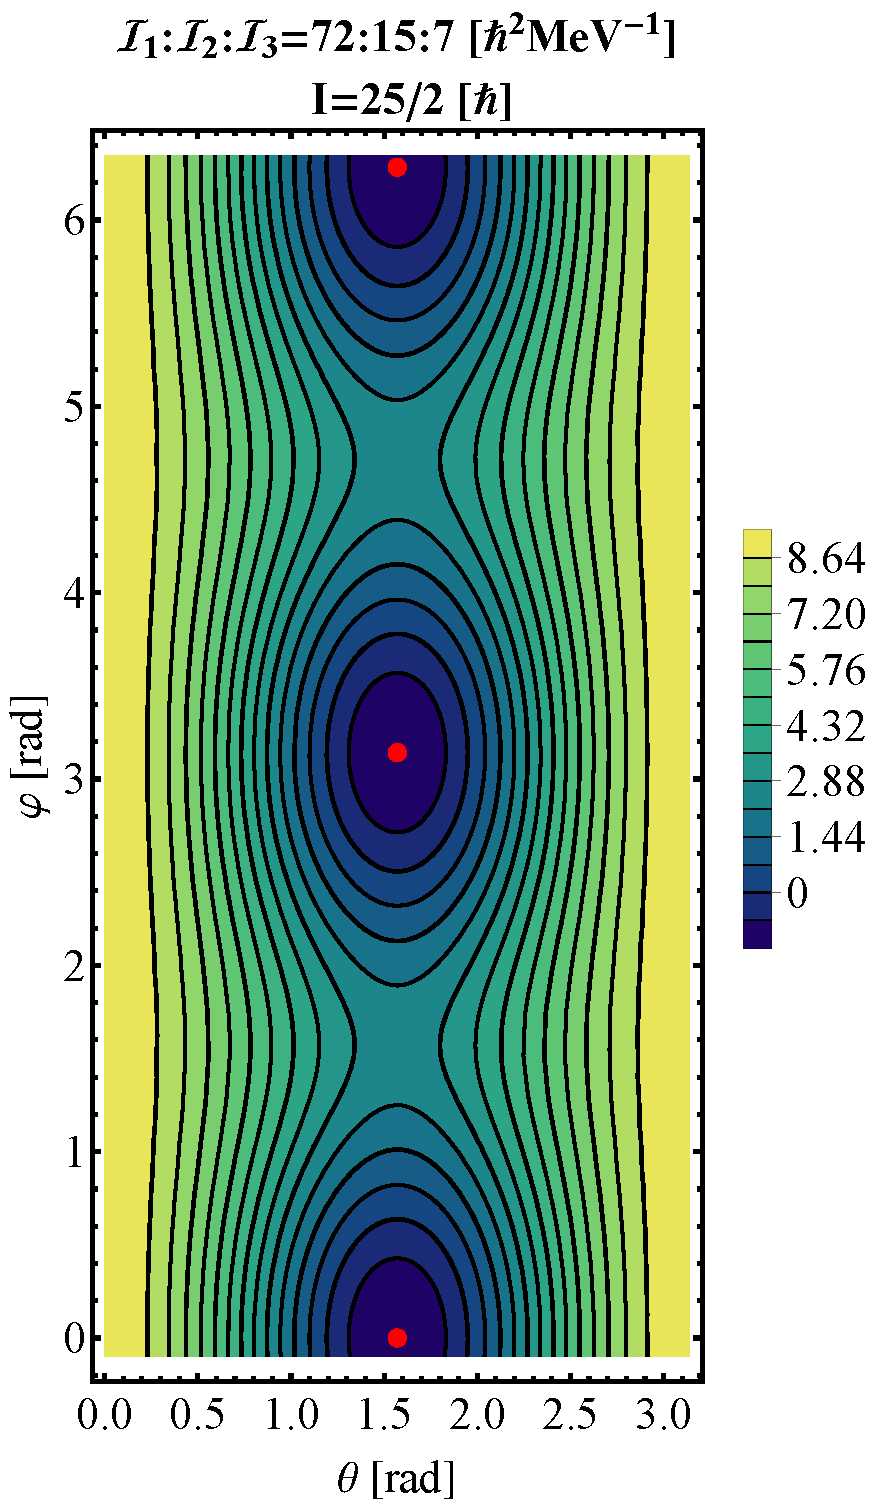
\includegraphics[scale=0.41]{figs/contour-tsd1.pdf}
\end{minipage}%
\begin{minipage}{.5\textwidth}
  \centering
 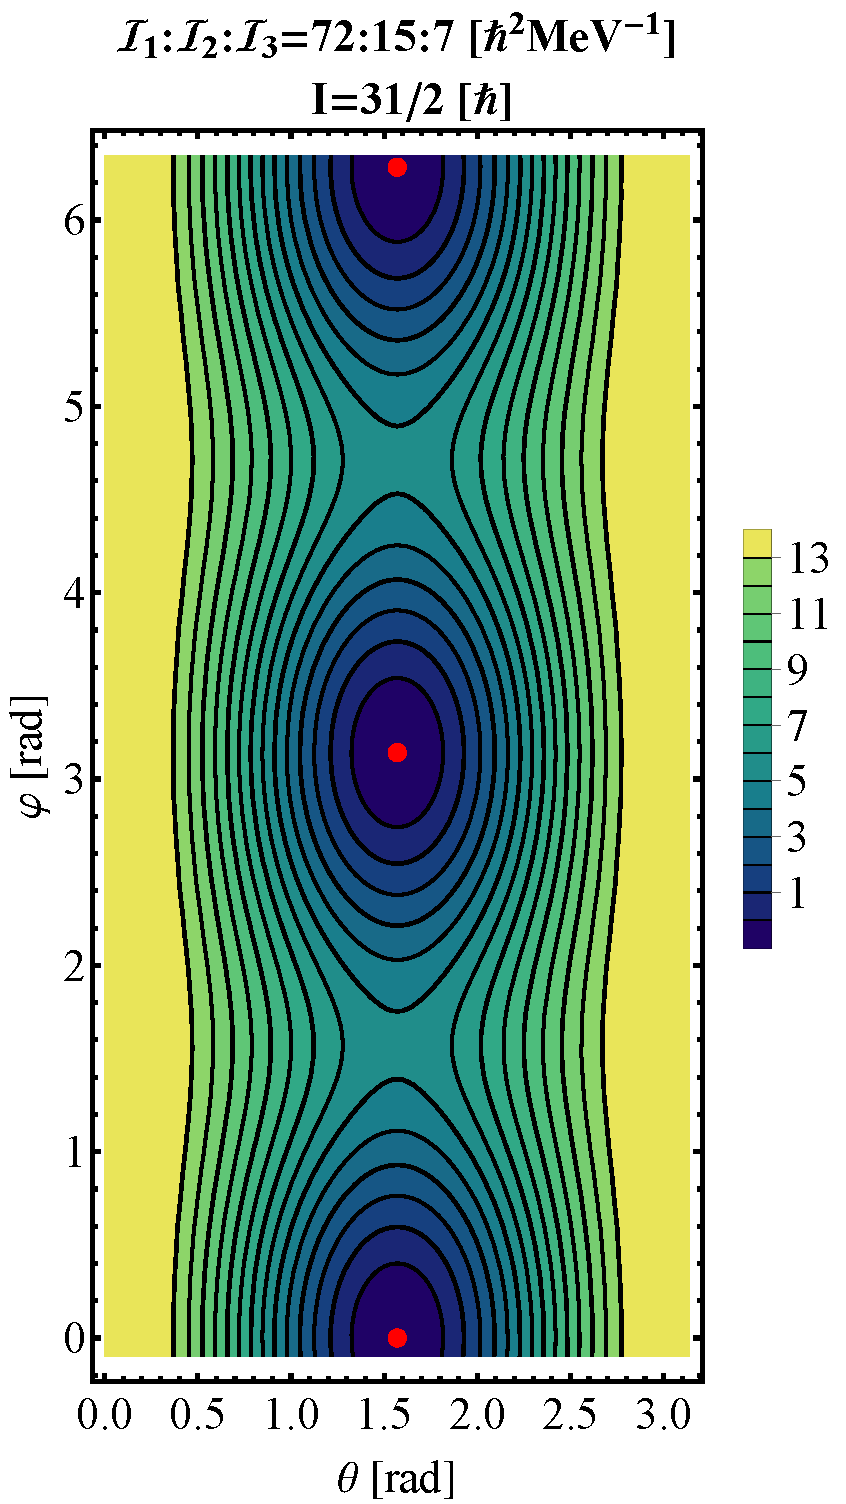
\includegraphics[scale=0.41]{figs/contour-tsd2.pdf}
\end{minipage}
\caption{Contour plots with the energy function $\mathcal{H}$ given by Eq. \ref{energy-function-minimal} for a state in $TSD_1$ (left) and a state from $TSD_2$ (right). Calculations were performed with the numerical parameters obtained from the fitting procedure of the excitation energies. The minimum points for $\mathcal{H}$ are marked by red dots, and they represent the regions in space where the nucleus has a stable wobbling character. The darker \emph{islands} also indicate a stable motion of the triaxial nucleus.}
    \label{contours-12}
\end{figure}

The four contour plots shown in Figures \ref{contours-12} and \ref{contours-34} have many similarities, suggesting common collective properties, but also differences which are caused by the fact that the minima have different depths. A common feature consists in that the equi-energy curves surround a sole minimum for low values in energy, but as the energy increases, the trajectories go around all minima, the lack of localization indicating unstable wobbling motion. The unstable regions might also relate to phase transitions, where the nucleus can undergo a major change in its rotational character. This aspect will also be discussed in the next subsection, devoted to the 3-dimensional representation of the energy ellipsoid and the classical trajectories of the triaxial system.

\begin{figure}
\centering
\begin{minipage}{.5\textwidth}
  \centering
  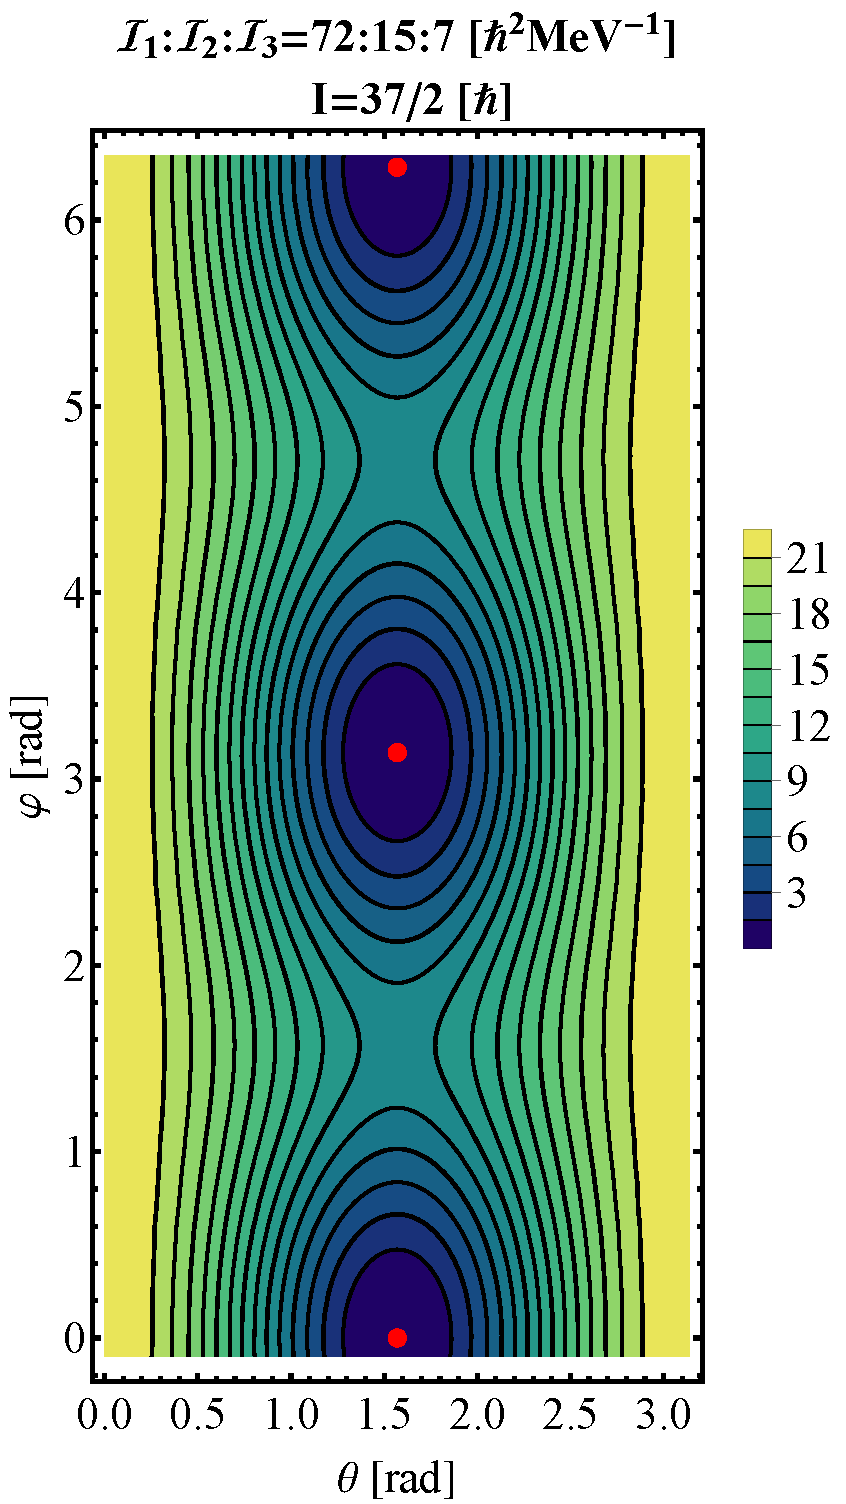
\includegraphics[scale=0.41]{figs/contour-tsd3.pdf}
\end{minipage}%
\begin{minipage}{.5\textwidth}
  \centering
 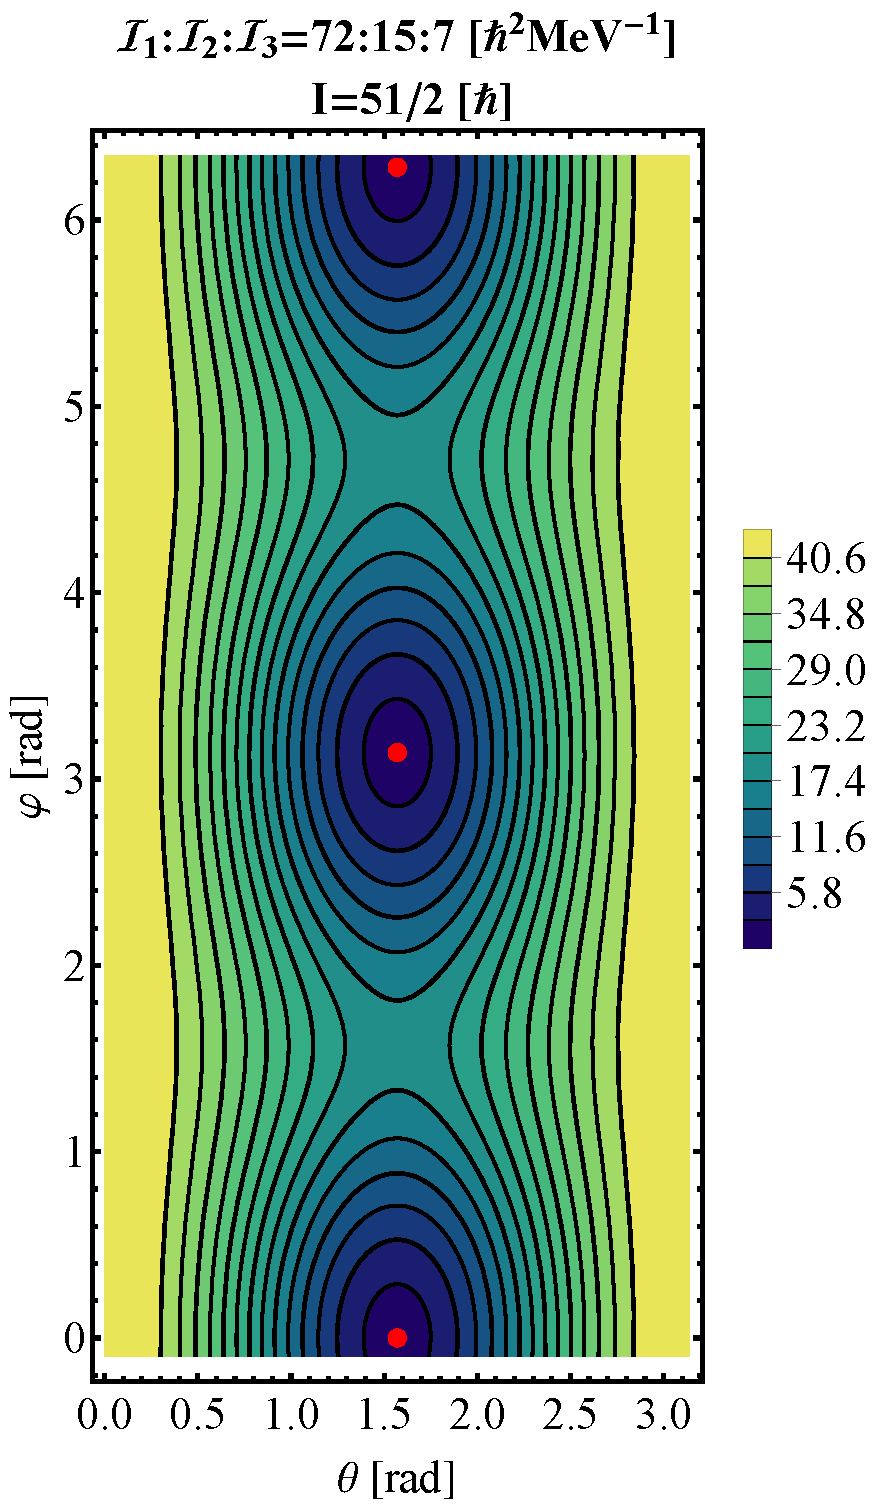
\includegraphics[scale=0.41]{figs/contour-tsd4.pdf}
\end{minipage}
\caption{Contour plots with the energy function $\mathcal{H}$ given by Eq. \ref{energy-function-minimal} for a state in $TSD_3$ (left) and a state from $TSD_4$ (right). Calculations were performed with the numerical parameters obtained from the fitting procedure of the excitation energies. The minimum points for $\mathcal{H}$ are marked by red dots, and they represent the regions in space where the nucleus has a stable wobbling character. The darker \emph{islands} also indicate a stable motion of the triaxial nucleus.}
    \label{contours-34}
\end{figure}

Regarding the minimum points (marked by red dots on the contour plots), their position remains unchanged for all four bands and any rotational state $I$, as long as the MOI order stays the same. Remarkable is the fact that only with the obtained set of parameters (the current MOI ordering) it was possible to define contours with stable motion (marked by the darker regions). Indeed, if the two ratios $\mathcal{I}_1/\mathcal{I}_2$ and $\mathcal{I}_2/\mathcal{I}_3$ would have been smaller, a larger unstable region would prevail (with islands of maximal character), constraining thus the stable wobbling motion. This could indicate the fact that the single-particle term $T_\text{s.p.}$ from $\mathcal{H}$ is sensitive to larger triaxiality, and only for certain values will the system achieve a stable motion characterized by large deformation (see Eq. \ref{energyfunction-core-single-particle-subterms}).

An additional step consists in the analysis of the energy function, more precisely to see its evolution in one of the minimum points with respect to the angular momentum $I$. As it was already observed from the contour plots shown in Figures \ref{contours-12}-\ref{contours-34}, the depth of the minima differs from one spin state to another, so it would be useful to have a quantitative view on that change. By fixing $\mathcal{H}$ in one of its critical points (e.g., the minimum $p_\text{min}(\theta,\varphi)=(\frac{\pi}{2},0)$), the angular momentum $I$ was varied within a large interval, and the evolution of $\mathcal{H}$ was evaluated. Graphical representation is shown in Figure \ref{energy-function-minimum-evolution}.

\begin{figure}
    \centering
    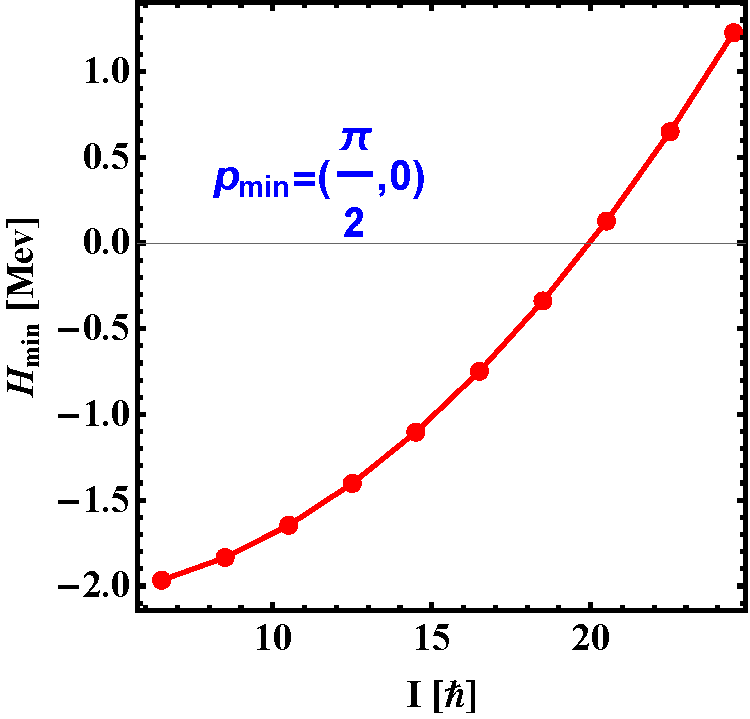
\includegraphics[scale=0.65]{figs/energy_function_minPoint_Evolution.pdf}
    \caption{The change in the minimum depth of $\mathcal{H}$, evaluated in the point $(\theta,\varphi)=(\frac{\pi}{2},0)$, for the obtained parameter set $\mathcal{P}$.}
    \label{energy-function-minimum-evolution}
\end{figure}

As it can be seen from Figure \ref{energy-function-minimum-evolution}, the classical energy $\mathcal{H}$ is an increasing function of angular momentum, which is to be expected, since the wobbling energies of the four bands increase with respect to the increase in spin. The negative values of $\mathcal{H}$ for low-lying wobbling states do not indicate that the nucleus has negative energy states since \emph{the rest} of the nucleus' energy is also given by the single-particle energy $\epsilon_j$ terms and the phononic $\mathcal{F}_{n_{w_1}n_{w_2}}^I$ terms.

Another useful insight would be the study of the classical energy function $\mathcal{H}$ for the obtained parameter set, as a function of the polar angles $(\theta,\varphi)$. This can be achieved by choosing a minimum point, keeping one of the polar coordinates fixed, and then let the other one vary across its corresponding interval. For $^{163}$Lu, such a graphical representation was done for the point $p_\text{min}=\left(\frac{\pi}{2},0\right)$ (that is the bottom-most red dot from each of the four contour plots depicted in Figures \ref{contours-12}-\ref{contours-34}). Results can be seen in Figure \ref{energy-function-min-point-evolution}.

\begin{figure}
\centering
\begin{minipage}{.5\textwidth}
  \centering
  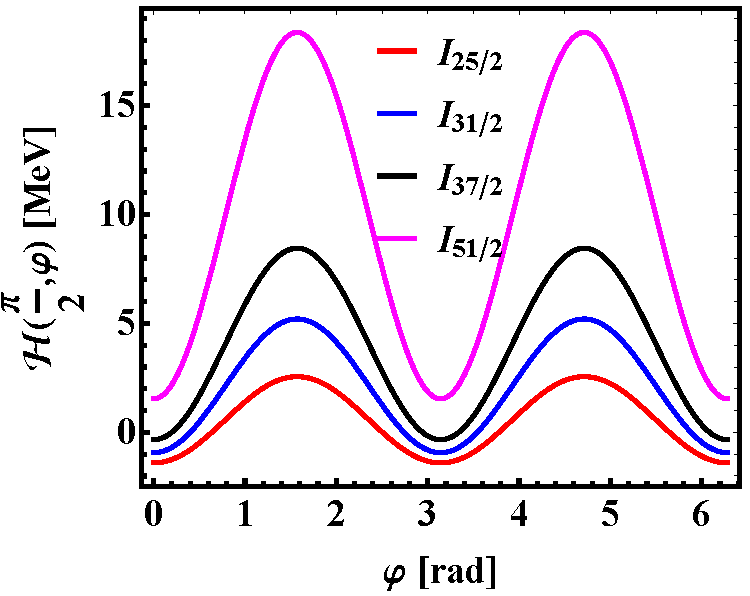
\includegraphics[scale=0.58]{figs/energyFunction_minTheta.pdf}
\end{minipage}%
\begin{minipage}{.5\textwidth}
  \centering
 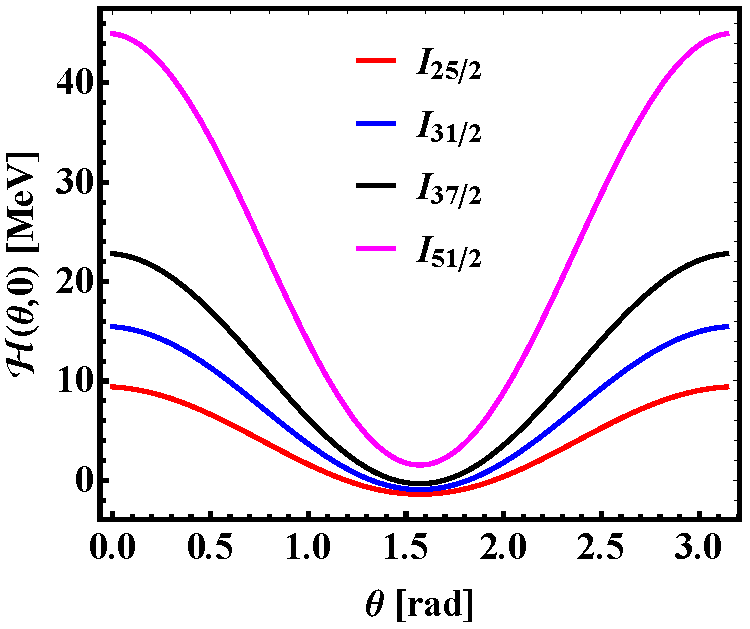
\includegraphics[scale=0.55]{figs/energyFunction_minVarphi.pdf}
\end{minipage}
\caption{The energy function $\mathcal{H}$, evaluated in one of its minimum points, as a function of the polar coordinates. One coordinate is fixed while the other one is varied within its interval of existence. For $\theta\in[0,\pi]$ and $\varphi\in[0,2\pi]$. The chosen minimum is $p_\text{min}=\left(\frac{\pi}{2},0\right)$. Each spin state corresponds to one of the four triaxial bands of $^{163}$Lu.}
    \label{energy-function-min-point-evolution}
\end{figure}


\subsection{Classical trajectories - 3-dimensional representation}\label{classical-trajectories}

The final step of the present work is to obtain an insight into the classical features of the $^{163}$ triaxial nucleus in terms of its motion within the angular momentum space. As already mentioned, the trajectories are given by the intersection curves of the energy ellipsoid $E$ given in Eq. \ref{energy-ellipsoid-cartesian} with the angular momentum sphere $I^2$ given in Eq. \ref{angular-momentum-sphere}. In the 3-dimensional space generated by the three components of the angular momentum vector $\vec{I}$, these intersection curves characterize the motion of the system, as each curve will be oriented along with one of the three axes $x_k\ ,\ k=1,2,3$, suggesting a rotational motion (the precession of the total a.m.) around a particular direction preferred by the system.

The dependence of the classical trajectories on the angular momenta as well as on energies is thus analyzed in $\texttt{W2}$. Indeed, when the model Hamiltonian is diagonalized for a given $I$, a set of $2I+1$ energies are obtained. Therefore, it is justified to study the evolution of trajectories when the energy of the nucleus is increasing. The curves are represented as the manifold given by the intersection of the two constants of motion, that is $E$ and $I^2$. An example of such trajectories are depicted in Figures \ref{trajectories-12}-\ref{trajectories-34}.

\begin{figure}
    \centering
    % 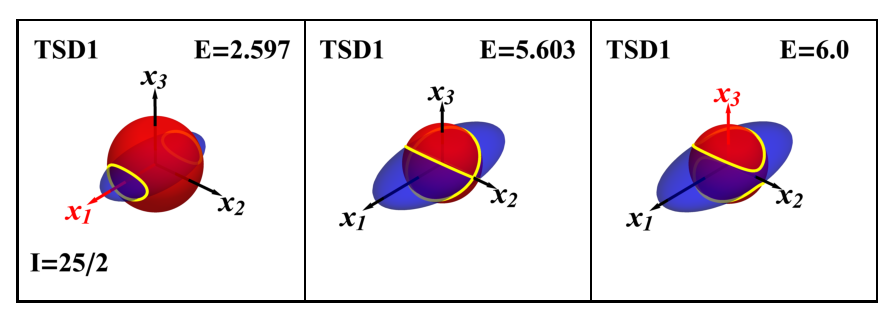
\includegraphics[width=0.8\textwidth]{figs/tsd1_spin1.eps}
    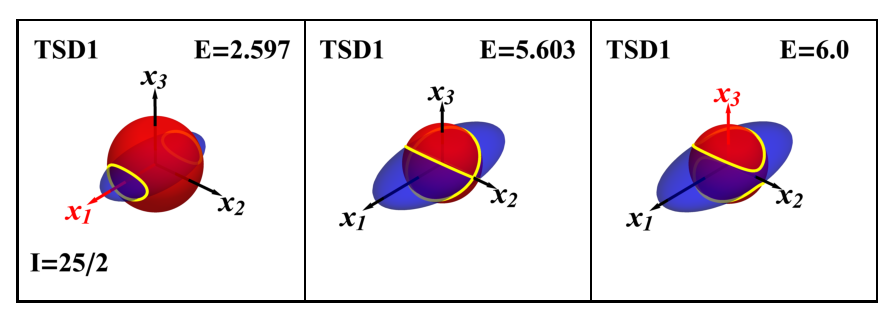
\includegraphics[scale=0.7]{figs/tsd1_spin1.eps}
    % 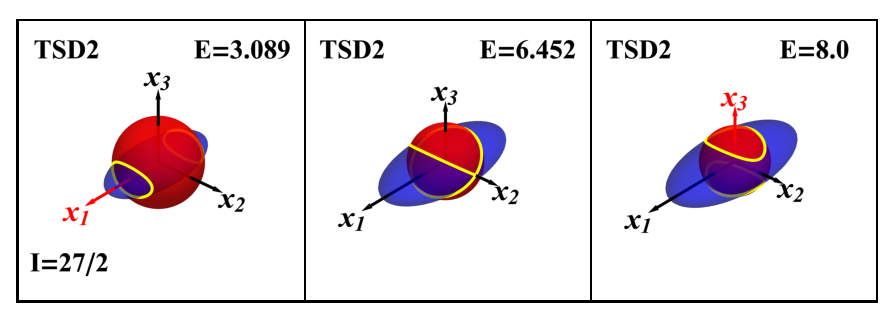
\includegraphics[width=0.8\textwidth]{figs/tsd2_spin1.eps}
    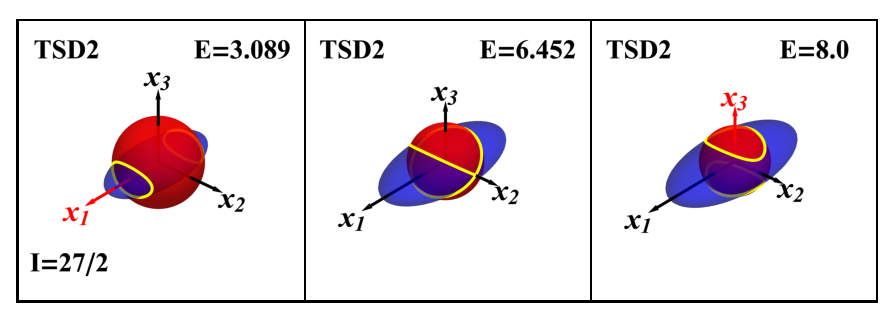
\includegraphics[scale=0.7]{figs/tsd2_spin1.eps}
    \caption{The nuclear trajectories of the system, evaluated for two spin states belonging to $TSD_1$ and $TSD_2$. Intersection lines marked by yellow color represents the actual orbits. Axis colored in red represents the direction along which the system rotates (it precesses). The left-most inset corresponds to the real excitation energy for that particular spin state $I$.}
    \label{trajectories-12}
\end{figure}


\begin{figure}
    \centering
    % 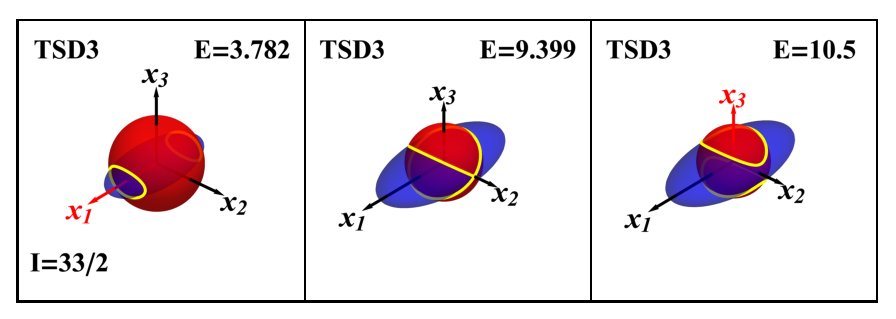
\includegraphics[width=0.8\textwidth]{figs/tsd3_spin1.eps}
    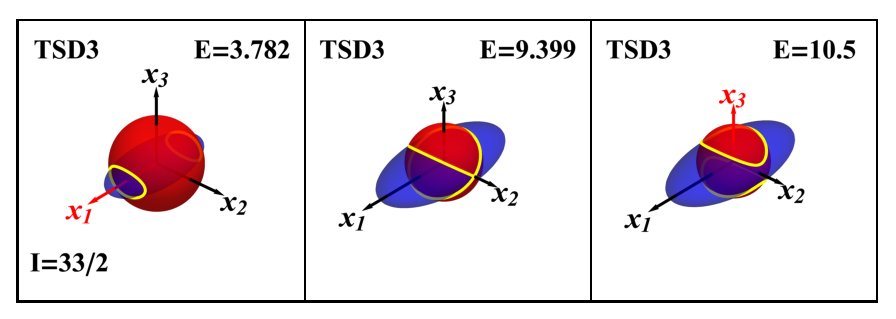
\includegraphics[scale=0.7]{figs/tsd3_spin1.eps}
    % 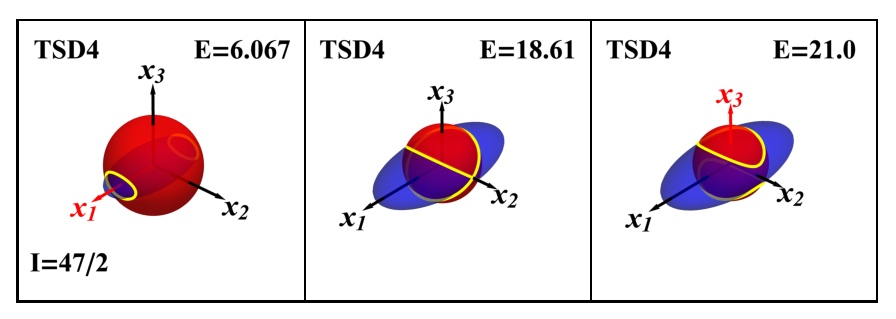
\includegraphics[width=0.8\textwidth]{figs/tsd4_spin1.eps}
    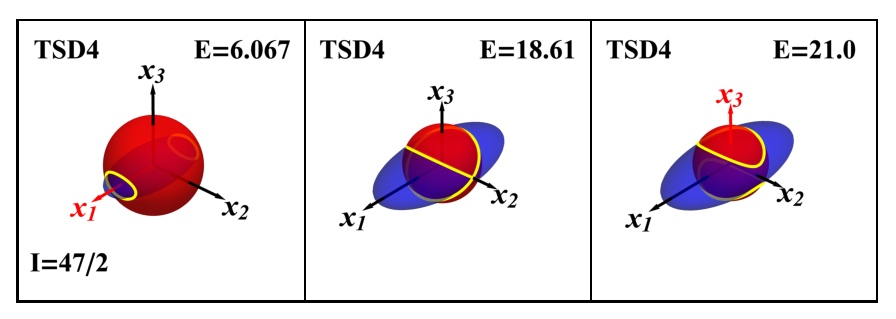
\includegraphics[scale=0.7]{figs/tsd4_spin1.eps}
    \caption{The nuclear trajectories of the system, evaluated for two spin states belonging to $TSD_3$ and $TSD_4$. Intersection lines marked by yellow color represents the actual orbits. Axis colored in red represents the direction along which the system rotates (it precesses). The left-most inset corresponds to the real excitation energy for that particular spin state $I$.}
    \label{trajectories-34}
\end{figure}

Each row from the Figures \ref{trajectories-12}-\ref{trajectories-34} represents a rotational state within a band. A low-lying spin state was chosen from each band in particular as an example. The left inset within each row represents the real excitation energy for the state $I$ at which the energy ellipsoid is evaluated. It can be seen that two distinct (but symmetric) trajectories are observed along the 1-axis, for all four states. This suggests that the states of the triaxial nucleus are obtained from the rotation of the angular momentum along $x_1$. Indeed, for low energies, the rotation is more pronounced along the $x_1$- and $-x_1$-axes. As the energy of the nucleus increases, the two trajectories approach each other, which results in a tilted rotation axis corresponding to both curves. The tilted axis implies that the rotation axis is being misaligned, the rotational axis moving away from its \emph{equilibrium point}, marking the tilted-axis-rotation. Note that this picture is fully consistent with the one described by Lawrie et al. \cite{lawrie2020tilted}. Further increase in energy will result in the two trajectories intersect with each other. That particular point where the intersection between the two orbits occurs is marked in the middle inset from each figure. Consequently, the intersection of these two orbits marks an unstable motion within the system. Finally, when the energy increases even more, beyond this \emph{critical point}, one arrives again in a two-trajectories regime but with a different rotation axis, lying closer to the $x_3$ axis. This case is shown in the right inset within each figure, where the axis $x_3$ is marked by red color, signaling the change in the rotational mode of the nucleus. However, it is worth noting that such energies are way too large for such a phase transition to occur naturally in $^{163}$Lu. For example, in the case of $I_{25/2}\in TSD_1$, the energy at which $^{163}$Lu undergoes a phase transition with regards to the rotational mode is close to $5.6\ \text{MeV}$ (middle inset for $TSD_1$ from Figure \ref{contours-12}), but the real excitation energy which corresponds to this state is half that (left inset for $TSD_1$ from Figure \ref{trajectories-12}). Nevertheless, it is a remarkable fact that with the current model, a phase transition between rotational modes in a triaxial nucleus can be identified. A proper microscopic formalism based on this current approach might also provide a more detailed picture with regards to the allowed trajectories for the system.


%\begin{table}[h!t]%
%\caption{This table is taken from RJP volume \textbf{50}(1-2) from page 43 (2005). It gives the ``
%\textit{number of bound states dependence on the radius of space curvature for $\alpha = 0.005$, $U_0 = 1$}''.}
%\centering
%\begin{tabular}{|c|c|}
%\hline
%Value $\rho$ & Value $\varepsilon$ \cr
%\hline
%$\rho = 50$ & -- \cr
%$\rho = 100$ & -- \cr
%$\rho = 250$ & $\varepsilon_1 = 0.0289$ \cr
%$\rho = 400$ & $\varepsilon_1 = 0.3772$ \cr
%$\rho = 1000$ & $\varepsilon_1 = 0.4142$, $\varepsilon_2 = 0.8495$ \cr
%\hline
%\end{tabular}
%\label{table1}
%\end{table}

\section{Conclusions \& Outlook}
\label{section-gata}

The purpose of the present work was two-fold. On one hand, a detailed overview regarding the current experimental observations for wobbling motion in both even- and odd-mass nuclei across several mass regions was made in the introductory part (covered in Section \ref{section2:expdata}). This was accompanied by a brief mention of the theoretical methods that are used for the microscopic/macroscopic description of the wobbling phenomenon (see Section \ref{section2:thmodels}). Also in the first part of the paper, a schematic analysis on the characteristics of the wobbling motion was made, which concerned the particle-core configurations in a longitudinal/transverse wobbler. Therein, it was shown that depending on the alignment of the odd quasiparticle with the triaxial core, a certain wobbling regime will prevail, thus concluding the introduction.

On the other hand, the second objective of the current paper was to extend a previous model that describes the $^{163}$Lu using a re-interpretation of its four wobbling bands $TSD_{1,2,3,4}$. The previous model (denoted here by \texttt{W1}) introduced the concept of signature partners between the bands $TSD_1$ and $TSD_2$. One showed that the nucleus can be described as a particle that is moving in a quadrupole deformed mean field generated by the core. In \texttt{W1}, there was an $i_{13/2}$ proton involved in the particle-rotor-coupling for the description of the first three triaxial bands, and another proton with negative parity, i.e., the $\pi(h_{9/2})$ intruder for band $TSD_4$. Based on $\texttt{W1}$, a new approach was developed here as an extension, denoted throughout the paper by $\texttt{W2}$. The new formalism starts with the same Hamiltonian, however, in the present case a single trial function is constructed to admit eigenstates with both positive and negative parity. Indeed, despite the fact that $TSD_4$ is of an opposite parity than the first three, all bands are described by the coupling of a unique single-particle ($i_{13/2}$ with positive parity $\pi_{j}=+1$) to the core states of positive parity for $TSD_{1,2,3}$ and core states of negative parity for $TSD_4$. The coupling schemes for the wobbling bands within \texttt{W2} were denoted throughout the paper by $C'_1, C'_2, C'_3$. From the quantal Hamiltonian specific to a Particle Rotor Model (given by Eq. \ref{prm-hamiltonian}), by applying a Time-Dependent Variational Principle (TDVE) as in Eq. \ref{tdve} with the trial function carefully chosen so that it allows a mixture of both positive and negative parity states, a set of analytical expressions for the excitation energies of each band were obtained (defined in Eq. \ref{wobbling_energies}). The excitation energies comprise a term that represents the classical energy function, obtained as the average of the Hamiltonian with the trial wave function (Eq. \ref{hmin:equation}). A second term has a phonon character (Eq. \ref{f-term}), being composed of two wobbling frequencies that were obtained from the solutions to a dispersion-like equation as defined in Eq. \ref{dispersion-eq}. 

From the theoretical formalism of the excitation energies of $^{163}$Lu, a set of free parameters emerged, containing the three moments of inertia, the single-particle potential strength $V$, and the triaxiality parameter $\gamma$. They were obtained through a fitting procedure which was done for all four bands, unlike the previous \texttt{W1} approach. The resulted parameter set provides an impressive agreement between the existing theoretical and experimental data concerning the wobbling spectrum of this isotope, with an r.m.s. of about $79\ \text{keV}$. An interpretation of the numerical values for the obtained parameters was done in Section \ref{results:interpret}, and indeed, the obtained values are consistent with other formalisms from the literature. Furthermore, the study of the classical energy function was done in a polar coordinate system, obtaining the contour plots for spin states belonging to each triaxial band (Section \ref{wobbling-stability}). The critical points from those contour maps indicate stability in terms of wobbling behavior (with closed orbits signaling stable trajectories). Unstable regions also emerge at high rotational energies. An additional comment on the wobbling nature of $^{163}$Lu was made (see Section \ref{wobbling-comment}), and an analysis of the wobbling energy behavior with spin showed that the increasing trend might indicate a longitudinal character. Lastly, by intersecting the angular momentum sphere with the energy ellipsoid, the classical trajectories can be obtained. The results of this 3-dimensional representation are discussed throughout Section \ref{classical-trajectories}. From the graphical illustrations, three situations might occur for any given spin state of $^{163}$Lu. i) At low energies, the rotation axis is either the $1$-axis or the $-1$-axis, resulting in two trajectories along this axis. ii) At a particular energy - \emph{critical energy} - the two orbits get close to each other until they intersect, marking the point of unstable motion for the nucleus. iii) If the energy increases even more, then the triaxial nucleus performs a tilted-axis-rotation, where the rotational axis slowly moves away from $x_1$, approaching $x_3$ and thus becoming misaligned. The change from one step to the other marks a phase transition. When the nucleus undergoes a transformation with regards to its rotational behavior it is actually changing its wobbling regime. Remarkable the fact that the current semi-classical approach is able to predict the change in the wobbling regime, this being of large interest in the nuclear community since evidence of such behavior was missing.

Concluding the present work, this newly developed formalism proves to be a successful tool for accurately describing the wobbling spectrum of $^{163}$Lu and also for providing an insight into the rotational motion of the nuclear system with respect to its total spin.


\begin{acknowledgement}
This work was supported by UEFISCU, through the project \textbf{PCE-16/2021}.
\end{acknowledgement}

\appendix
\section{Appendix - Workflow Diagrams}
\label{appendix:a}
The two models described in Section 2, namely the formalism $\texttt{W1}$ (see Section \ref{subsection:w1}) and \texttt{W2} (see Section \ref{subsection:w2}) are schematically represented, based on the discussions made for each of the two approaches. The \texttt{W1} mode corresponds to the work given in Refs. \cite{raduta2020approach,raduta2020towards}, and the \texttt{W2} corresponds to the formalism developed in the present paper. For the formalism \texttt{W1}, the diagram is shown in Figure \ref{w1-model-worfklow}, while for the newly developed approach \texttt{W2}, the diagram is shown in Figure \ref{w2-model-worfklow}.

%\subsection{The \texttt{W1} model}
\begin{figure}
    \centering
    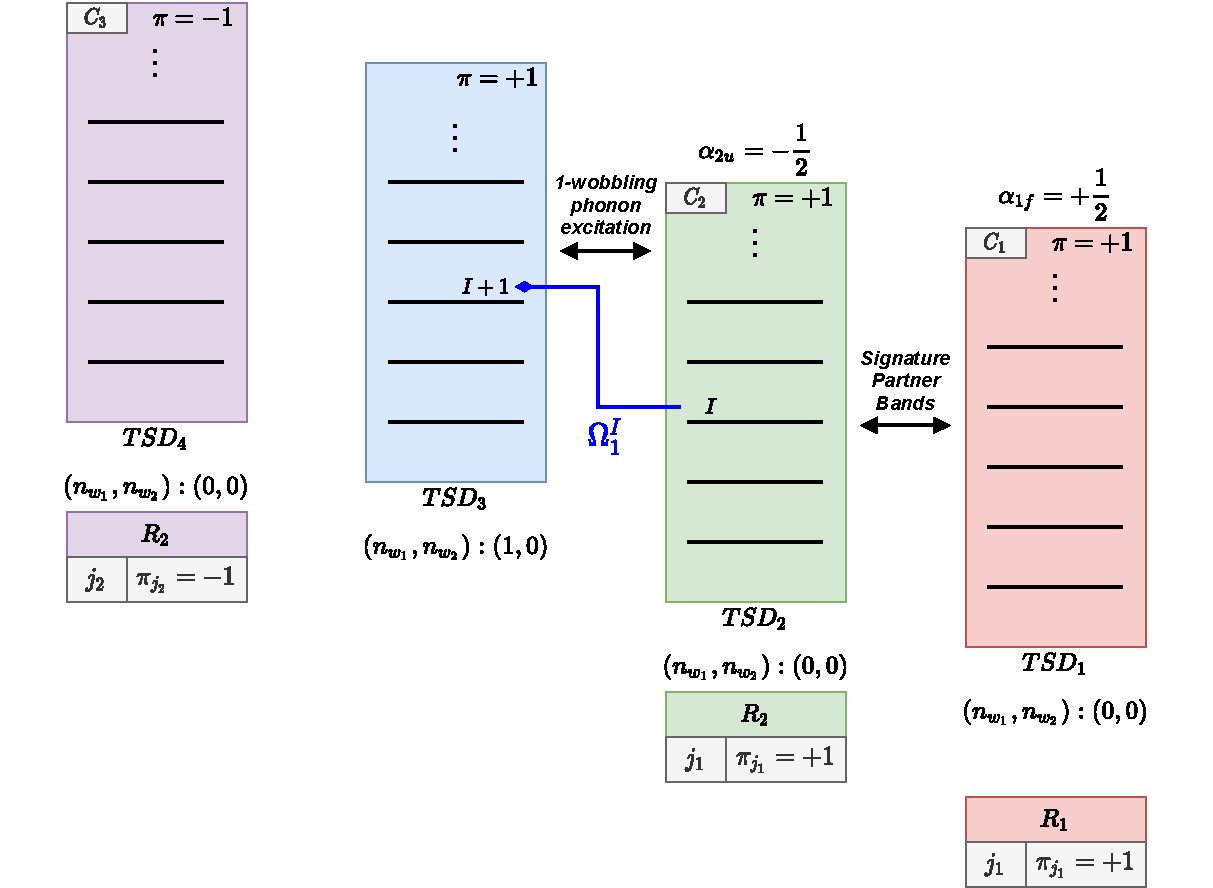
\includegraphics[scale=0.8]{figs/W1_Approach.pdf}
    \caption{Schematic representation of the band structure adopted for $^{163}$Lu in the \texttt{W1} model. For each band, the wobbling phonon numbers are shown. The main features and linking properties between bands are represented with arrows. The bottom part shows the coupling scheme (the core and the valence nucleon) for each wobbling band as described in the text, namely $C_1$, $C_2$, $C_3$ (see Section \ref{subsection:w1}). The blue arrow marks the activation of $TSD_3$ states via the phonon operator.}
    \label{w1-model-worfklow}
\end{figure}
%\subsection{The \texttt{W2} model}
\begin{figure}
   \centering
    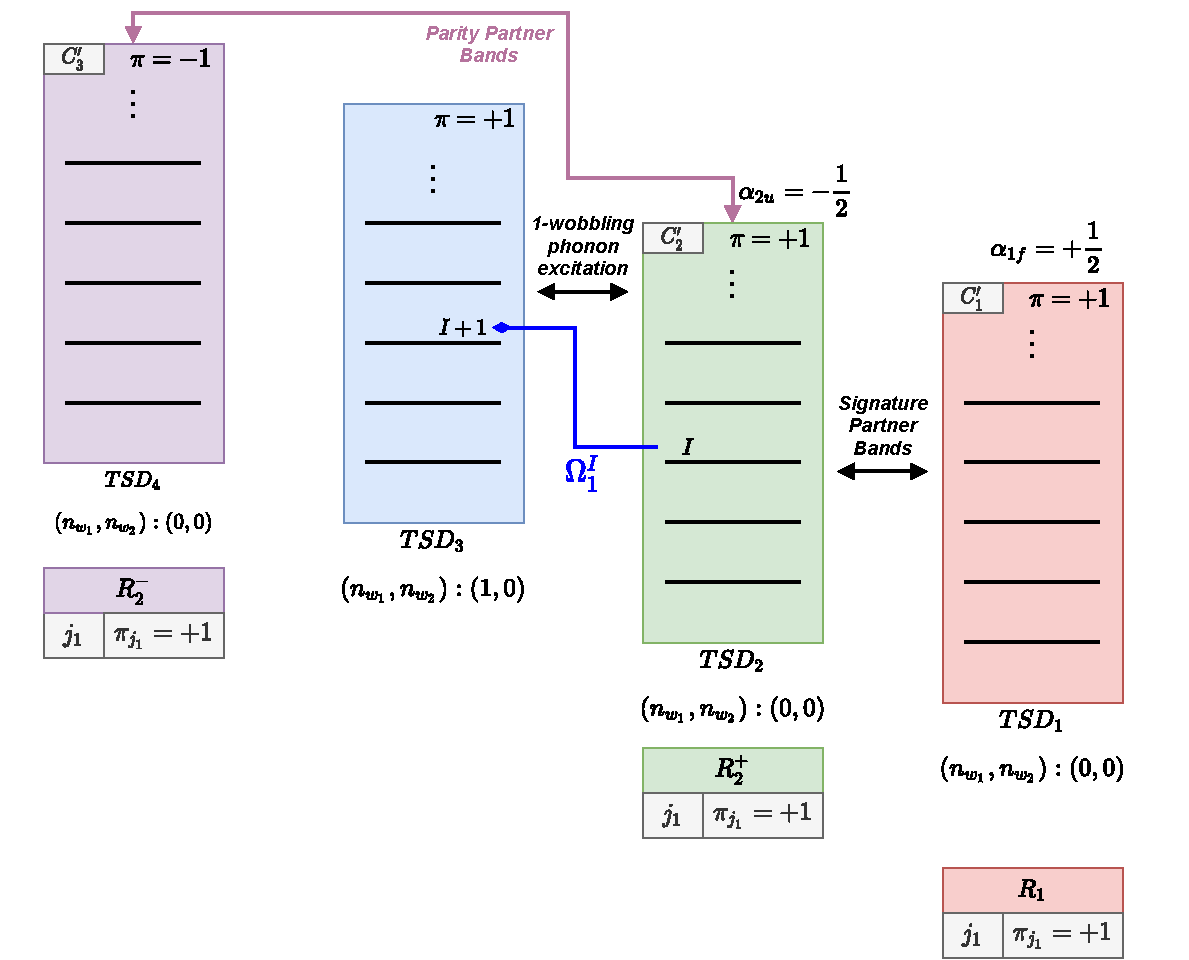
\includegraphics[scale=0.8]{figs/W2_Approach.pdf}
    \caption{Schematic representation of the band structure adopted for $^{163}$Lu in the \texttt{W2} model. For each band, the wobbling phonon numbers are shown. The main features and linking properties between bands are represented with arrows. The bottom part shows the coupling scheme (the core and the valence nucleon) for each wobbling band as described in the text, namely $C'_1$, $C'_2$, $C'_3$. The blue arrow marks the activation of $TSD_3$ states via the phonon operator.}
    \label{w2-model-worfklow}
\end{figure}

\newpage

\begin{thebibliography}{99}

\bibitem{moller2006global}
Peter M{\"o}ller, Ragnar Bengtsson, B~Gillis Carlsson, Peter Olivius, and
  Takatoshi Ichikawa.
\newblock{\em Physical review letters}, 97(16):162502, 2006.

\bibitem{moller2009heavy}
Peter M{\"o}ller, Arnold~J Sierk, Takatoshi Ichikawa, Akira Iwamoto, Ragnar
  Bengtsson, Henrik Uhrenholt, and Sven {\AA}berg.
\newblock{\em Physical Review C}, 79(6):064304, 2009.

\bibitem{hamamoto1988triaxial}
I~Hamamoto and H~Sagawa.
\newblock{\em Physics Letters B}, 201(4):415--419, 1988.

\bibitem{bengtsson1984signature}
R~Bengtsson, H~Frisk, FR~May, and JA~Pinston.
\newblock{\em Nuclear Physics A}, 415(2):189--214, 1984.

\bibitem{stachel1982triaxiality}
J~Stachel, N~Kaffrell, E~Grosse, H~Emling, H~Folger, R~Kulessa, and D~Schwalm.
\newblock{\em Nuclear Physics A}, 383(3):429--467, 1982.

\bibitem{frauendorf1997tilted}
Stefan Frauendorf and Jie Meng.
\newblock{\em Nuclear Physics A}, 617(2):131--147, 1997.

\bibitem{bohr1998nuclear}
Aage~Niels Bohr and Ben~R Mottelson.
\newblock{\em Nuclear Structure (In 2 Volumes)}.

\bibitem{xiong2019nuclear}
BW~Xiong and YY~Wang.
\newblock{\em Atomic Data and Nuclear Data Tables}, 125:193--225, 2019.

\bibitem{dimitrov2000chirality}
VI~Dimitrov, S~Frauendorf, and F~D{\"o}nau.
\newblock{\em Physical review letters}, 84(25):5732, 2000.

\bibitem{koike2003systematic}
T~Koike, K~Starosta, CJ~Chiara, DB~Fossan, and DR~LaFosse.
\newblock{\em Physical Review C}, 67(4):044319, 2003.

\bibitem{meng2006possible}
J~Meng, J~Peng, SQ~Zhang, and S-G Zhou.
\newblock{\em Physical Review C}, 73(3):037303, 2006.

\bibitem{raduta2016new}
AA~Raduta, Al~H Raduta, and CM~Petrache.
\newblock{\em Journal of Physics G: Nuclear and Particle Physics},
  43(9):095107, 2016.

\bibitem{petrache2018evidence}
CM~Petrache, BF~Lv, A~Astier, E~Dupont, YK~Wang, SQ~Zhang, PW~Zhao, ZX~Ren,
  J~Meng, PT~Greenlees, et~al.
\newblock{\em Physical Review C}, 97(4):041304, 2018.

\bibitem{lv2019chirality}
BF~Lv, CM~Petrache, QB~Chen, J~Meng, A~Astier, E~Dupont, P~Greenlees, H~Badran,
  T~Calverley, DM~Cox, et~al.
\newblock{\em Physical Review C}, 100(2):024314, 2019.

\bibitem{raduta2020towards}
AA~Raduta, R~Poenaru, and CM~Raduta.
\newblock{\em Journal of Physics G: Nuclear and Particle Physics},
  47(2):025101, 2020.

\bibitem{hagemann2003quantized}
Gudrun~B Hagemann and Ikuko Hamamoto.
\newblock{\em Nuclear Physics News}, 13(3):20--24, 2003.

\bibitem{odegaard2001evidence}
SW~{\O}deg{\aa}rd, GB~Hagemann, DR~Jensen, M~Bergstr{\"o}m, B~Herskind,
  G~Sletten, S~T{\"o}rm{\"a}nen, JN~Wilson, PO~Tj{\o}m, I~Hamamoto, et~al.
\newblock{\em Physical review letters}, 86(26):5866, 2001.

\bibitem{jensen2002evidence}
DR~Jensen, GB~Hagemann, I~Hamamoto, SW~{\O}deg{\aa}rd, B~Herskind, G~Sletten,
  JN~Wilson, K~Spohr, H~H{\"u}bel, P~Bringel, et~al.
\newblock{\em Physical review letters}, 89(14):142503, 2002.

\bibitem{jensen2002wobbling}
D~Ringk{\o}bing Jensen, GB~Hagemann, I~Hamamoto, SW~{\O}deg{\aa}rd,
  M~Bergstr{\"o}m, B~Herskind, G~Sletten, S~T{\"o}rm{\"a}nen, JN~Wilson,
  PO~Tj{\o}m, et~al.
\newblock{\em Nuclear Physics A}, 703(1-2):3--44, 2002.

\bibitem{schnack1995superdeformed}
H~Schnack-Petersen, Ragnar Bengtsson, RA~Bark, P~Bosetti, A~Brockstedt,
  H~Carlsson, LP~Ekstr{\"o}m, GB~Hagemann, B~Herskind, F~Ingebretsen, et~al.
\newblock{\em Nuclear Physics A}, 594(2):175--202, 1995.

\bibitem{biswas2019longitudinal}
S~Biswas, R~Palit, S~Frauendorf, U~Garg, W~Li, GH~Bhat, JA~Sheikh, J~Sethi,
  S~Saha, Purnima Singh, et~al.
\newblock{\em The European Physical Journal A}, 55(9):1--7, 2019.

\bibitem{matta2017transverse}
James~Till Matta.
\newblock Transverse wobbling in 135 pr.
\newblock In {\em Exotic Nuclear Excitations: The Transverse Wobbling Mode in
  135 Pr}, pages 77--93. Springer, 2017.


\bibitem{sensharma2019two}
N~Sensharma, U~Garg, S~Zhu, AD~Ayangeakaa, S~Frauendorf, W~Li, GH~Bhat,
  JA~Sheikh, MP~Carpenter, QB~Chen, et~al.
\newblock{\em Physics Letters B}, 792:170--174, 2019.

\bibitem{chakraborty2020multiphonon}
S~Chakraborty, HP~Sharma, SS~Tiwary, C~Majumder, AK~Gupta, P~Banerjee,
  S~Ganguly, S~Rai, S~Kumar, A~Kumar, et~al.
\newblock{\em Physics Letters B}, 811:135854, 2020.

\bibitem{petrache_2018}
C~M Petrache.
\newblock{\em LNL Annual Report}, 2018.

\bibitem{timar2019experimental}
J~Tim{\'a}r, QB~Chen, B~Kruzsicz, D~Sohler, I~Kuti, SQ~Zhang, J~Meng, P~Joshi,
  R~Wadsworth, K~Starosta, et~al.
\newblock{\em Physical review letters}, 122(6):062501, 2019.

\bibitem{nandi2020first}
S~Nandi, G~Mukherjee, QB~Chen, S~Frauendorf, R~Banik, Soumik Bhattacharya,
  Shabir Dar, S~Bhattacharyya, C~Bhattacharya, S~Chatterjee, et~al.
\newblock{\em Physical Review Letters}, 125(13):132501, 2020.

\bibitem{sensharma2020longitudinal}
N~Sensharma, U~Garg, QB~Chen, S~Frauendorf, DP~Burdette, JL~Cozzi, KB~Howard,
  S~Zhu, MP~Carpenter, P~Copp, et~al.
\newblock{\em Physical review letters}, 124(5):052501, 2020.

\bibitem{guo2020risk}
S~Guo, XH~Zhou, CM~Petrache, EA~Lawrie, S~Mthembu, YD~Fang, HY~Wu, HL~Wang,
  HY~Meng, GS~Li, et~al.
\newblock{\em arXiv preprint arXiv:2011.14354}, 2020.

\bibitem{hamilton2010super}
JH~Hamilton, SJ~Zhu, YX~Luo, AV~Ramayya, S~Frauendorf, JO~Rasmussen, JK~Hwang,
  SH~Liu, GM~Ter-Akopian, AV~Daniel, et~al.
\newblock{\em Nuclear Physics A}, 834(1-4):28c--31c, 2010.

\bibitem{luo2013triaxial}
YX~Luo, JH~Hamilton, AV~Ramaya, JK~Hwang, SH~Liu, JO~Rasmussen, S~Frauendorf,
  GM~Ter-Akopian, AV~Daniel, Yu~Ts Oganessian, et~al.
\newblock Triaxial and triaxial softness in neutron rich ru and pd nuclei.
\newblock In {\em Exotic Nuclei: EXON-2012}, pages 215--224. World Scientific,
  2013.


\bibitem{petrache2019diversity}
CM~Petrache, PM~Walker, S~Guo, QB~Chen, S~Frauendorf, YX~Liu, RA~Wyss,
  D~Mengoni, YH~Qiang, A~Astier, et~al.
\newblock{\em Physics Letters B}, 795:241--247, 2019.

\bibitem{wang2020two}
YK~Wang, FQ~Chen, and PW~Zhao.
\newblock{\em Physics Letters B}, 802:135246, 2020.

\bibitem{chen2019transverse}
QB~Chen, S~Frauendorf, and CM~Petrache.
\newblock{\em Physical Review C}, 100(6):061301, 2019.

\bibitem{frauendorf2014transverse}
S~Frauendorf and F~D{\"o}nau.
\newblock{\em Physical Review C}, 89(1):014322, 2014.

\bibitem{hamamoto2002wobbling}
Ikuko Hamamoto.
\newblock{\em Physical Review C}, 65(4):044305, 2002.

\bibitem{tanabe2006algebraic}
Kosai Tanabe and Kazuko Sugawara-Tanabe.
\newblock{\em Physical Review C}, 73(3):034305, 2006.

\bibitem{wen2015wobbling}
Shi Wen-Xian and Chen Qi-Bo.
\newblock{\em Chinese Physics C}, 39(5):054105, 2015.

\bibitem{davydov1958rotational}
AS~Davydov and GF~Filippov.
\newblock{\em Nuclear Physics}, 8:237--249, 1958.

\bibitem{shimizu1995nuclear}
Yoshifumi~R Shimizu and Masayuki Matsuzaki.
\newblock{\em Nuclear Physics A}, 588(3):559--596, 1995.

\bibitem{matsuzaki2002wobbling}
Masayuki Matsuzaki, Yoshifumi~R Shimizu, and Kenichi Matsuyanagi.
\newblock{\em Physical Review C}, 65(4):041303, 2002.

\bibitem{matsuzaki2003dynamical}
Masayuki Matsuzaki, Yoshifumi~R Shimizu, and Kenichi Matsuyanagi.
\newblock{\em The European Physical Journal A-Hadrons and Nuclei},
  20(1):189--190, 2003.

\bibitem{matsuzaki2004instability}
Masayuki Matsuzaki and Shin-Ichi Ohtsubo.
\newblock{\em Physical Review C}, 69(6):064317, 2004.

\bibitem{matsuzaki2004nuclear}
Masayuki Matsuzaki, Yoshifumi~R Shimizu, and Kenichi Matsuyanagi.
\newblock{\em Physical Review C}, 69(3):034325, 2004.

\bibitem{shimizu2005high}
Yoshifumi~R Shimizu, Masayuki Matsuzaki, and Kenichi Matsuyanagi.
\newblock{\em Physical Review C}, 72(1):014306, 2005.

\bibitem{shimizu2008parametrizations}
Yoshifumi~R Shimizu, Takuya Shoji, and Masayuki Matsuzaki.
\newblock{\em Physical Review C}, 77(2):024319, 2008.

\bibitem{shoji2009microscopic}
Takuya Shoji and Yoshifumi~R Shimizu.
\newblock{\em Progress of theoretical physics}, 121(2):319--355, 2009.

\bibitem{chen2014collective}
QB~Chen, SQ~Zhang, PW~Zhao, and J~Meng.
\newblock{\em Physical Review C}, 90(4):044306, 2014.

\bibitem{chen2016wobbling}
QB~Chen, SQ~Zhang, J~Meng, et~al.
\newblock{\em Physical Review C}, 94(5):054308, 2016.

\bibitem{mukhopadhyay2007chiral}
S~Mukhopadhyay, D~Almehed, U~Garg, S~Frauendorf, T~Li, PV~Madhusudhana Rao,
  X~Wang, SS~Ghugre, MP~Carpenter, S~Gros, et~al.
\newblock{\em Physical review letters}, 99(17):172501, 2007.

\bibitem{qi2009chirality}
Bin Qi, SQ~Zhang, J~Meng, SY~Wang, and S~Frauendorf.
\newblock{\em Physics Letters B}, 675(2):175--180, 2009.

\bibitem{oi2000wobbling}
Makito Oi, Ahmad Ansari, Takatoshi Horibata, and Naoki Onishi.
\newblock{\em Physics Letters B}, 480(1-2):53--60, 2000.

\bibitem{raduta2017semiclassical}
AA~Raduta, R~Poenaru, and L~Gr Ixaru.
\newblock{\em Physical Review C}, 96(5):054320, 2017.

\bibitem{raduta2020new}
AA~Raduta, CM~Raduta, and R~Poenaru.
\newblock{\em Journal of Physics G: Nuclear and Particle Physics},
  48(1):015106, 2020.

\bibitem{tanabe1971triaxiality}
K~Tanabe and K~Sugawara-Tanabe.
\newblock{\em Physics Letters B}, 34(7):575--578, 1971.

\bibitem{tanabe2008selection}
Kosai Tanabe and Kazuko Sugawara-Tanabe.
\newblock{\em Physical Review C}, 77(6):064318, 2008.

\bibitem{shimada2018rotational}
Mitsuhiro Shimada, Yudai Fujioka, Shingo Tagami, and Yoshifumi~R Shimizu.
\newblock{\em Physical Review C}, 97(2):024318, 2018.

\bibitem{hara1995projected}
Kenji Hara and Yang Sun.
\newblock{\em International Journal of Modern Physics E}, 4(04):637--785,
  1995.

\bibitem{zhao2016configuration}
PW~Zhao, P~Ring, and J~Meng.
\newblock{\em Physical Review C}, 94(4):041301, 2016.

\bibitem{konieczka2018gamow}
M~Konieczka, Markus Kortelainen, and W~Satu{\l}a.
\newblock{\em Physical Review C}, 97(3):034310, 2018.

\bibitem{raduta2007semiclassical}
AA~Raduta, R~Budaca, and CM~Raduta.
\newblock{\em Physical Review C}, 76(6):064309, 2007.

\bibitem{raduta2018wobbling}
AA~Raduta, R~Poenaru, and Al~H Raduta.
\newblock{\em Journal of Physics G: Nuclear and Particle Physics},
  45(10):105104, 2018.

\bibitem{budaca2018tilted}
R~Budaca.
\newblock{\em Physical Review C}, 97(2):024302, 2018.

\bibitem{raduta2020approach}
AA~Raduta, R~Poenaru, and CM~Raduta.
\newblock{\em Physical Review C}, 101(1):014302, 2020.

\bibitem{bengtsson1990high}
Tord Bengtsson.
\newblock{\em Nuclear Physics A}, 512(1):124--148, 1990.

\bibitem{gorgen2004quadrupole}
A~G{\"o}rgen, RM~Clark, M~Cromaz, P~Fallon, GB~Hagemann, H~H{\"u}bel, IY~Lee,
  AO~Macchiavelli, G~Sletten, D~Ward, et~al.
\newblock{\em Physical Review C}, 69(3):031301, 2004.

\bibitem{hagemann2005triaxiality}
GB~Hagemann.
\newblock{\em Acta Physica Polonica B}, 36(4):1043, 2005.

\bibitem{jensen2004coexisting}
DR~Jensen, GB~Hagemann, I~Hamamoto, B~Herskind, G~Sletten, JN~Wilson,
  SW~{\O}deg{\aa}rd, K~Spohr, H~H{\"u}bel, P~Bringel, et~al.
\newblock{\em The European Physical Journal A-Hadrons and Nuclei},
  19(2):173--185, 2004.

\bibitem{tanabe2017stability}
Kosai Tanabe and Kazuko Sugawara-Tanabe.
\newblock{\em Physical Review C}, 95(6):064315, 2017.

\bibitem{frauendorf2018comment}
S~Frauendorf.
\newblock{\em Physical Review C}, 97(6):069801, 2018.

\bibitem{tanabe2018reply}
Kosai Tanabe and Kazuko Sugawara-Tanabe.
\newblock{\em Physical Review C}, 97(6):069802, 2018.

\bibitem{sun1994varied}
Yang Sun, Shuxian Wen, et~al.
\newblock{\em Physical Review C}, 50(5):2351, 1994.

\bibitem{khalaf11properties}
AM~Khalaf, Hayam Yassin, and Eman R~Abo Elyazeed.
\newblock{\em Journal: Journal Of Advances In Physics}, 11(1), 2015.

\bibitem{uma2015deltai}
VS~Uma and Alpana Goel.
\newblock{\em The European Physical Journal Plus}, 130(6):1--6, 2015.

\bibitem{mittal2016signature}
HM~Mittal and Anshul Dadwal.
\newblock In {\em Proceedings of the DAE-BRNS Symp. on Nucl. Phys}, volume~61,
  page 134, 2016.

\bibitem{hamamoto1983intrinsic}
Ikuko Hamamoto and Ben Mottelson.
\newblock{\em Physics Letters B}, 127(5):281--285, 1983.

\bibitem{hamamoto1987rotational}
Ikuko Hamamoto.
\newblock{\em Physics Letters B}, 193(4):399--404, 1987.

\bibitem{hamamoto2016interplay}
Ikuko Hamamoto.
\newblock{\em Physica Scripta}, 91(2):023004, 2016.

\bibitem{torilov2004spectroscopy}
S~Torilov, S~Thummerer, W~Von~Oertzen, Tz~Kokalova, G~De~Angelis, HG~Bohlen,
  A~Tumino, M~Axiotis, E~Farnea, N~Marginean, et~al.
\newblock{\em The European Physical Journal A-Hadrons and Nuclei},
  19(3):307--317, 2004.

\bibitem{debray2000alternating}
ME~Debray, MA~Cardona, D~Hojman, AJ~Kreiner, M~Davidson, J~Davidson, H~Somacal,
  G~Levinton, DR~Napoli, S~Lenzi, et~al.
\newblock{\em Physical Review C}, 62(2):024304, 2000.

\bibitem{radutaa2009csm}
AA~Radutaa and CM~Radutab.
\newblock{\em arXiv preprint arXiv:0903.0076}, 2009.

\bibitem{raduta2011simultaneous}
AA~Raduta and CM~Raduta.
\newblock{\em Annals of the University of Craiova, Physics}, 21(1):28--53,
  2011.

\bibitem{meyer1975collective}
J~Meyer-ter Vehn.
\newblock{\em Nuclear Physics A}, 249(1):111--140, 1975.

\bibitem{wang2008description}
SY~Wang, SQ~Zhang, B~Qi, J~Peng, JM~Yao, J~Meng, et~al.
\newblock{\em Physical Review C}, 77(3):034314, 2008.

\bibitem{peng2003description}
J~Peng, J~Meng, and SQ~Zhang.
\newblock{\em Physical Review C}, 68(4):044324, 2003.

\bibitem{koike2004chiral}
T~Koike, K~Starosta, and I~Hamamoto.
\newblock{\em Physical review letters}, 93(17):172502, 2004.

\bibitem{wang2007doublet}
SY~Wang, SQ~Zhang, B~Qi, and J~Meng.
\newblock{\em Physical Review C}, 75(2):024309, 2007.

\bibitem{reich2010nuclear}
CW~Reich and Balraj Singh.
\newblock{\em Nuclear Data Sheets}, 111(5):1211--1469, 2010.

\bibitem{chasman1980incipient}
RR~Chasman.
\newblock{\em Physics Letters B}, 96(1-2):7--10, 1980.

\bibitem{raduta2006description}
AA~Raduta, CM~Raduta, and Amand Faessler.
\newblock{\em Physics Letters B}, 635(2-3):80--84, 2006.

\bibitem{raduta2006simultaneous}
AA~Raduta, Al~H Raduta, and CM~Raduta.
\newblock{\em Physical Review C}, 74(4):044312, 2006.

\bibitem{shou2009coupling}
Wang Shou-Yu, Qi~Bin, and Zhang Shuang-Quan.
\newblock{\em Chinese Physics Letters}, 26(5):052102, 2009.

\bibitem{lawrie2020tilted}
EA~Lawrie, O~Shirinda, and CM~Petrache.
\newblock{\em Physical Review C}, 101(3):034306, 2020.

\end{thebibliography}



\end{document}